
\chapter{Irradiation of pulmonary veins under influence of respiration in human data}
\label{chapter:mdacc}
\minitoc


PVs move due to the heartbeat and respiration of the patient. Both motion types are independent from each other and can hence be studied 
individually. While the influence of heartbeat is analyzed in chapter \ref{chapter:human}, the effect of respiratory motion will be discussed 
in this chapter. 4DCTs of nine lung cancer patients were recorded for cancer radiotherapy at MD Anderson Cancer Center in Houston (MDACC, 
Texas, USA) where patients were treated with proton therapy and IMRT. The same data has been used in previous studies on motion mitigation 
techniques using carbon ion beams (e.g. \cite{Lue12, Woe11}). The PV were contoured and the resulting motion pattern, direction as well as 
motion amplitude of LPV and RPV due to respiration were studied for all cases. Respiration is also a problematic factor for catheter ablation 
as it can cause changes in catheter contact force and hence alter the result \cite{Kum12}. For the proposed non-invasive treatment modality 
with a scanned carbon ion beam the respiratory motion will endanger the treatment outcome as it often leads to inhomogeneous dose coverage. Hence 
motion mitigation techniques are needed. The resulting interplay pattern for all patients as well as gating as a possible motion mitigation 
technique have been studied and the results will be presented in this chapter. Exemplary for two patient cases rescanning inside the gating 
window was analyzed. 

\section{Material and methods}
Details on the input data as well as the used treatment planning parameters will be given. Afterwards an overview on all 
studies will be presented and the analysis procedure will be described.  

\vspace*{-0.3cm}
\subsection{Treatment planning input data}
For treatment planning studies with the in-house treatment planning software TRiP4D \cite{Ric13}, 4DCT data sets, target and OAR contours as 
well as a deformable image registration for motion assessment in-between the different motion phases are needed. Details on the used 
input data as well as the used treatment planning parameters will be given.\newline 
\newline
In order to assess the motion of the PV due to respiration, lung cancer patient data was used. The 4DCTs of nine patients were recorded and 
anonymized at MDACC. Each of the 4DCT data consisted of ten motion phases, the reference phase was 
motion phase five at end exhale. The amplitude of the respiratory motion was assessed by measuring the difference between the (right) diaphragmatic dome in-between 
end exhale and end inhale on a frontal view of the 4DCT data. The amplitudes in the superior-inferior (SI) motion direction, the 
largest motion component in case of respiration, ranged from 2.5mm to 25mm (CT slice distance and hence resolution of 2.5mm). The varying 
motion amplitudes are displayed for all patients in 
table \ref{tab:patdata}. Two of the nine patients (patient 6 and 7) displayed a very shallow breathing with an amplitude of less than 5mm. 
Five patients (patient 1 to 5) had a breathing amplitude between 10mm and 20mm in SI direction. Two patients (patient 8 and 9) were breathing 
deeply with an amplitude bigger than 20mm. This indicates different breathing patterns as well as varying lung volume 
expansion and hence heart displacement amongst the studied patients. 

% \vspace*{-0.3cm}

\begin{table}[H]
  \centering
%   \footnotesize
  \caption{Respiratory motion in the direction of the largest motion component (SI) for all investigated patients. Furthermore the lung tumor 
  location (left lung (L) or right lung (R)) is stated next to the tumor volume.}
  \begin{tabular}{|c|c|c|c|}
    \hline\hline
    patient no & motion [mm] & tumor volume [cm$^{3}$] & tumor location (L/R)\\
    \hline
    1 & 17.5 & 236.5 & L \\
    2 & 20 & 572.2 & R \\
    3 & 10 & 160.2 & R \\
    4 & 17.5 & 676.1 & L \\
    5 & 15 & 372.1 & R \\
    6 & 2.5 & 706.1 & R \\
    7 & 5 & 123.8 & L \\
    8 & 25 & 44.7 & L \\
    9 & 22.5 & 125.3 & L \\
    \hline\hline
  \end{tabular}
  \label{tab:patdata}
\end{table}

\newpage

Segmentation of the LPV and RPV was performed with an in-house display functionality for TRiP \cite{Hil09}. Its graphical interface 
allows contouring on the axial slices of the reference phase of the 4DCT. The contours were checked and validated by a medical physicist 
who was involved in the animal studies of Sharma et al. \cite{Sha10} as well as a cardiologist from Mayo Clinic. Only the motion influence 
and the motion mitigation possibilities will be studied here, hence contouring of other volumes or organs at risk was omitted. A detailed 
analysis of the dose to the organs at risk in human data is performed in chapter \ref{chapter:human}. The volumes of the contours for the 
ablation sites for LPV and RPV are presented for each patient in table \ref{tab:volume}. 

\begin{table}[H]
  \centering
%   \footnotesize
  \caption{Target volume for LPV and RPV for all investigated patients.}
  \begin{tabular}{|c|c|c|}
    \hline\hline
    patient no & LPV [cm$^{3}$] & RPV [cm$^{3}$]\\
    \hline
    1 & 1.88 & 5.26 \\
    2 & 3.57 & 4.79 \\
    3 & 6.49 & 11.52 \\
    4 & 3.66 & 3.87 \\
    5 & 2.07 & 4.37 \\
    6 & 3.40 & 6.34 \\
    7 & 4.29 & 6.23 \\
    8 & 6.89 & 4.84 \\
    9 & 2.92 & 2.56 \\
    \hline\hline
  \end{tabular}
  \label{tab:volume}
\end{table}

Non-rigid image registration of the nine motion phases on the reference phase have been performed with Plastimatch \cite{Sharp07, Shack10}. 
A B-spline registration with the following parameters was chosen: The first step was carried out with 50 maximal iterations and an isotropic 
spacing of 35mm between the control points of the B-spline grid. In the second step, with 100 maximal iterations, the grid 
spacing was set to 11mm and the regularization to $\lambda$=0.005. 
The quality of registration was validated with visualization techniques: false color images \cite{Bro07}, checker board images 
\cite{Bro07} as well as a qualitative check of the vector field regularization. These tests were carried out between the two most extreme 
motion phases: the reference phase at end exhale (motion phase five) and the phase at end inhale (motion phase zero).


\subsection{Treatment planning parameters}
\label{mdacc:tpp}
Treatment plans without motion (3D, static) as well as with motion (4D) were generated. 
For the dose optimization process, 3D treatment plans were generated to homogeneously cover the CTVs in the reference phase while 4D treatment
plans covered the ITV \cite{Gra12}, which was generated from all twenty motion phases. 
Besides the original volume of the CTV safety margins have been added to the volumes of the treatment planning study. These margins were applied 
in order to account for possible deviations in between treatment planning and delivery, like positioning errors, changes 
between CT acquisition and treatment delivery etc. Isotropic safety margins of 3mm, 5mm and 7mm have been chosen. The ITV volumes used as the 
final PTV target were generated from the original CTV contour as well as the CTVs with margin, so that potential range variations were 
considered in the margins.\newline
\newline
The grid spacing was chosen to be 1$\mathrm{mm}$, both in $x$ and $y$ direction. The spacing between the IESs were chosen to be 3 mm$_{H2O}$. 
A maximal contour extension\footnote{determines the extent of rasterpoint positions outside the target contour} of 1.1 times the focal 
spot size of 4mm was chosen as well as a distal contour fall off of 4mm$_{H2O}$. TRiP's 'all points divergent beam' algorithm was used to 
calculate the absorbed dose. All treatment plans were calculated as intensity modulated particle therapy (IMPT). 
Following Sharma et al. \cite{Sha10} a physical dose of 25Gy was applied in one fraction in all simulations.\newline
\newline
Three different beam entrance directions were used. For all beam directions the couch was rotated by 90$^{\circ}$ while the 
gantry angles were set to -45$^{\circ}$, 135$^{\circ}$ and 0$^{\circ}$, respectively. With these field number and directions a good sparing 
of normal tissue, especially of the coronary arteries as well as of the aorta and of the trachea could be obtained (see chapter \ref{chapter:human}). 
The field directions were validated by a cardiologist from Mayo Clinic.\newline
\newline
The generation of treatment plans is furthermore also dependent on the theoretically possible 
beam application. Spill length, shape and particle intensity are thus important factors. For the here presented simulations HIT accelerator 
parameters have been used. Thereby a spill length of up to 5s is assumed. The pause in between spills has a mean value of 4.5s. The spill 
shape is rectangular. The particle intensities at HIT used for treatment planning vary between 5x10$^{6}$ and 8x10$^{7}$ particles per spill. 
Inbetween these two extreme intensity levels, eight different intensity levels can be used. In the resulting treatment plan, the intensity 
steps are automatically chosen \cite{Krae00, Ric13}. The minimum particle number per beam spot was set to 11,000.\newline
\newline
As the reconstruction of the 4DCTs was based on the time scale a phase-based motion state detection was employed. 
A Lujan motion type was chosen for the motion trajectories \cite{Luj99}. In order to consider possible divergence in the respiratory motion 
pattern of patients, different periods (6s and 8s) as well as different starting phases (0$^{\circ}$ and 90$^{\circ}$) were used. 
The motion periods were chosen according to the respiratory rate of 8 to 10 cycles per minute. 

\newpage

\subsection{Treatment planning studies}

3D treatment plans on the CTV volume were produced as reference values to the 4D cases, as it represents the ideal but not deliverable dose 
distribution. Different ITV margins (original and increased with 3mm, 5mm and 7mm margin) were studied for all patients in the 4D treatment plans. 
In order to prepare for these 4D simulations, the motion of the PVs due to respiration was assessed. 
4D plans were distinguished between an underlying motion without any compensation, resulting in interplay patterns \cite{Phi92, Ber08}, 
and with the application of gating \cite{Kub96} as motion mitigation technique. The gating window was set to 30\% around end exhale (reference 
phase five), so that motion phases four, five and six were used. For two patient cases (patient 2 and 9) rescanning inside the gating window 
was furthermore studied. Thereby four different rescan numbers (five, ten, fifteen and twenty rescans) have been studied. Treatment plans for 
all patients where carried out with one beam channel combination (couch angle of 90$^{\circ}$ and gantry angles of -45$^{\circ}$, 
135$^{\circ}$ and 0$^{\circ}$), all four safety margins, the stated treatment planning parameters and the four stated motion trajectories. 


\subsection{Analysis}

For comparison of the resulting dose coverage dose-volume-histograms (DVHs) were studied. The V95 (measure of dose coverage) and V107 (measure 
of over dosage) of the CTVs were analyzed. As an indicator for the dose homogeneity, the width of the dose fall off was determined by analyzing 
the difference D5-D95. The stated values have been evaluated for all beam application techniques (static, interplay, gating, rescanning within 
gating window). Furthermore motion-volume-histograms (MVHs) were generated in order to assess the resulting motion of the PV due to respiration. \newline
\newline
In order to study correlations between the diaphragm motion and the motion of the PVs the Pearson coefficient $r$ was determined and 
is reported for limits of $p$<0.05. Furthermore the relation of dose analysis parameters to different margin sizes and the studied irradiation 
technique was analyzed by a one-way analysis of variance (one-way ANOVA) and the proportion of variance explained ($r^{2}$ - which ranges from 
zero (fit has no predictive value) to one) and is reported with the corresponding p-value ($p$<0.0001). \newline
\newline
Boxplots of dose analysis parameters D5-D95 and V95 over all patient data sets, motion patterns and target volumes were moreover generated 
in order to study the influence of margin size and irradiation mode (static, interplay and gating). Thereby the median (50th 
percentile) as well as the 25th and 75th percentile are displayed next to the minimum and maximum. 
 

\newpage

\section{Results}

In the following the results of the motion assessment as well as of the treatment planning studies for all studied cases 
(static, interplay and gating as well as rescanning within the gating window) will be presented.  
The expected treatment time will be discussed. 


\subsection{Motion assessment of respiration}
\label{motion}
Using the resulting deformation maps from deformable image registration the motion of the ablation sites of LPV and RPV was assessed. Motion 
volume histograms (MVHs) \cite{Ric13} displaying the relative displacement of every voxel of the investigated volume to the reference phase 
in all three motion directions (SI: superior-inferior, AP: anterior-posterior, LR: left-right) as well as the absolute displacement (ABS) 
were generated. The mean and standard deviation of these displacement values in each motion phase of LPV and RPV are plotted for all patients 
and motion directions in figure \ref{motion_resp_all_lpv} and \ref{motion_resp_all_rpv}, respectively. The numerical values can be found 
in appendix \ref{app:mdacc:motion}. \newline
\newline
The mean and standard deviation of the displacement between the two extreme motion phases (end exhale and end inhale) are shown for all 
patients in tables \ref{tab:motion:LPV:mdacc} and \ref{tab:motion:RPV:mdacc} for the different motion directions and for the two target volumes, LPV and 
RPV, respectively. 
Depending on the patient the absolute displacement of the pulmonary veins were found to vary between three millimeters and more than 
one centimeter. From the nine studied patients patient 9 is displaying the highest absolute displacement, both in LPV and RPV.
For all patients, the largest motion direction is SI, resulting in the largest contribution to the absolute displacement. The 
average in SI direction over the entire volume reaches up to 15.5mm (average over all patients of (6.8 $\pm$ 3.8)mm) for LPV and 10.9mm 
(average over all patients of (6.8 $\pm$ 2.5)mm) for RPV. The other two motion directions show a much smaller displacement. In AP direction the maximal 
motion is less than 2.5mm (standard deviation of less than 1mm) and in LR the PVs move less than 2.7mm (standard deviation of 1mm).
Over all patients, the mean absolute displacement in-between end exhale and end inhale of the LPV is (6.8 $\pm$ 3.6)mm and 
(6.8 $\pm$ 2.5)mm for RPV. For the SI direction, the mean displacement over all patients is (-6.4 $\pm$ 3.8)mm for LPV and (-6.6 $\pm$ 2.4)mm for 
RPV.\newline
\newline
It can furthermore be seen that the relative displacement of the target volumes around end exhale (motion phase five, reference phase) is small 
for all motion directions and patients. The difference between motion phase four and six was only 3mm in the absolute displacement 
of patient 9, which is the patient with the largest motion in the patient cohort. Hence gating around end exhale was expected to be an 
adequate motion mitigation technique for the irradiation of the PVs under influence of respiration. 


%%%%%%%%%%% MVHs %%%%%%%%%%%%%%%%

\newpage

\begin{figure}[H]
\begin{center}
 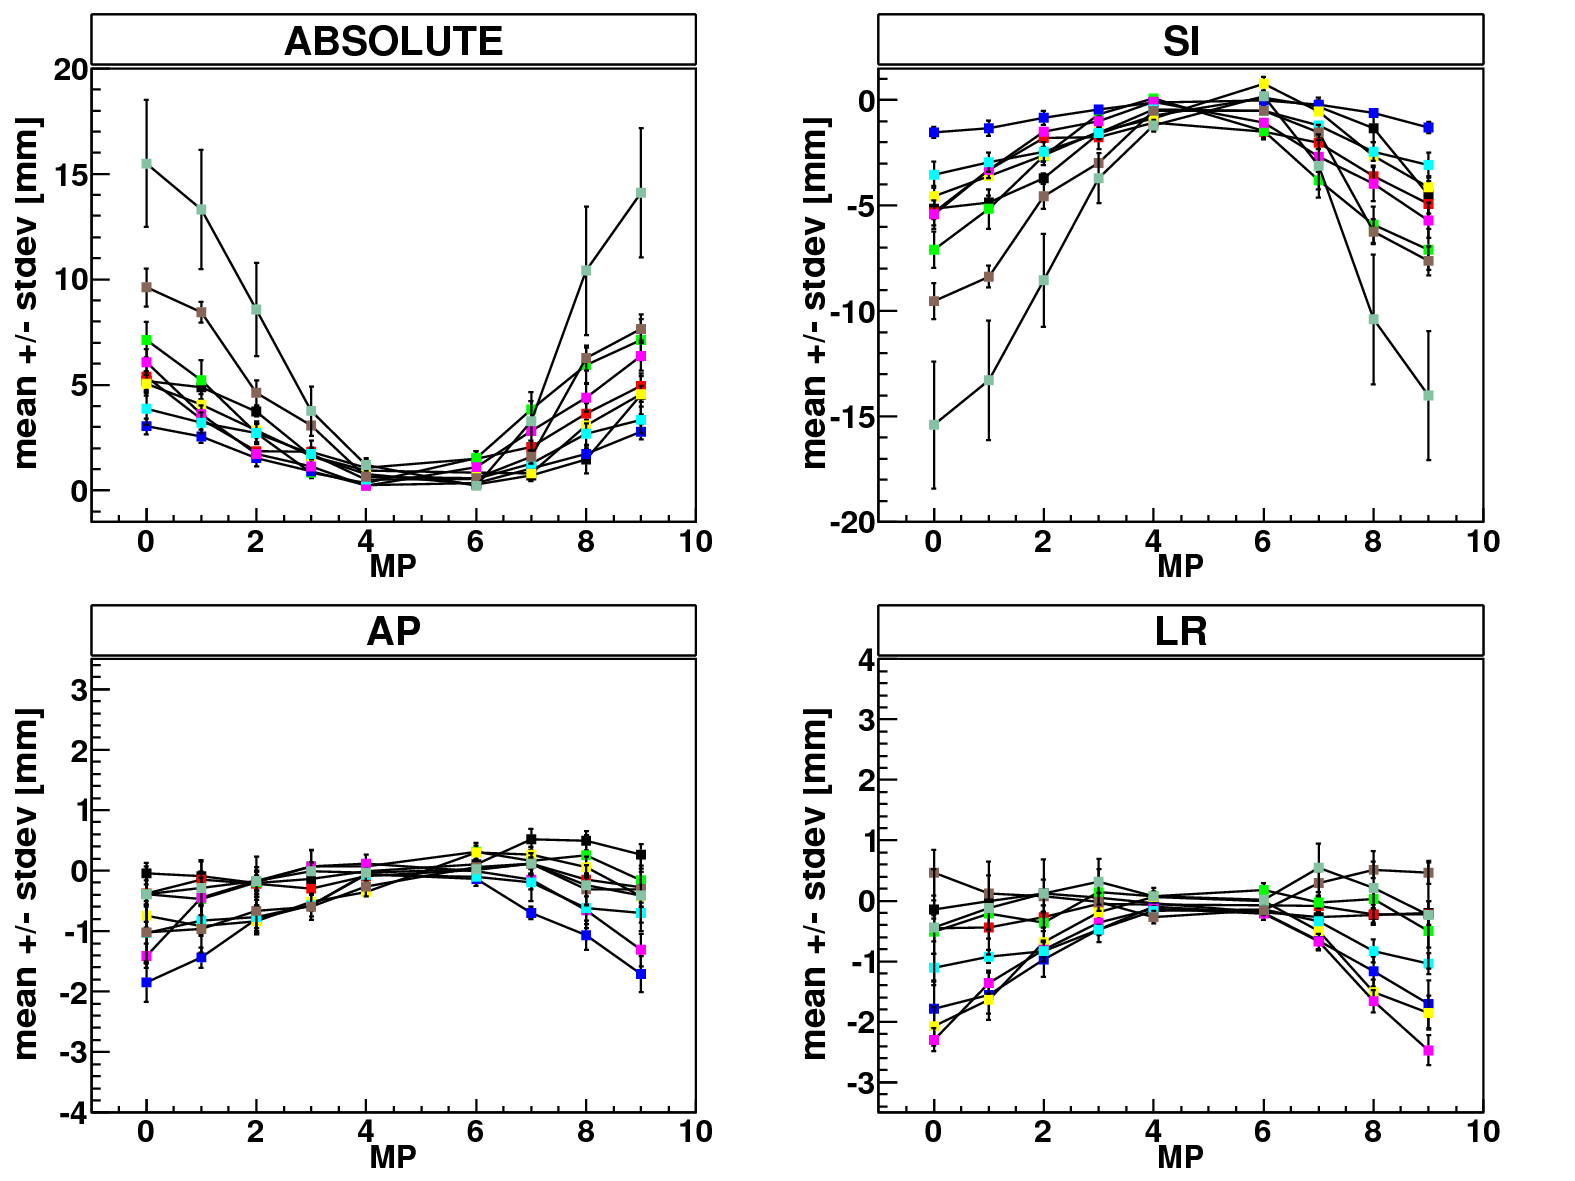
\includegraphics[scale=0.22]{./teile/results_mdacc/MDACC_allPatients_RESP_LPV.png}
\caption{LPV: Mean motion amplitude and standard deviation in each motion phase (MP) relative to the reference phase under influence of 
respiration for all patients (patient 1: black, patient 2: red, patient 3: green, patient 4: blue, patient 5: yellow, patient 6: pink, patient 
7: turquois, patient 8: brown, patient 9: olive). }
\label{motion_resp_all_lpv}
\end{center}
\end{figure}

\vspace*{-1cm}

\begin{figure}[H]
\begin{center}
 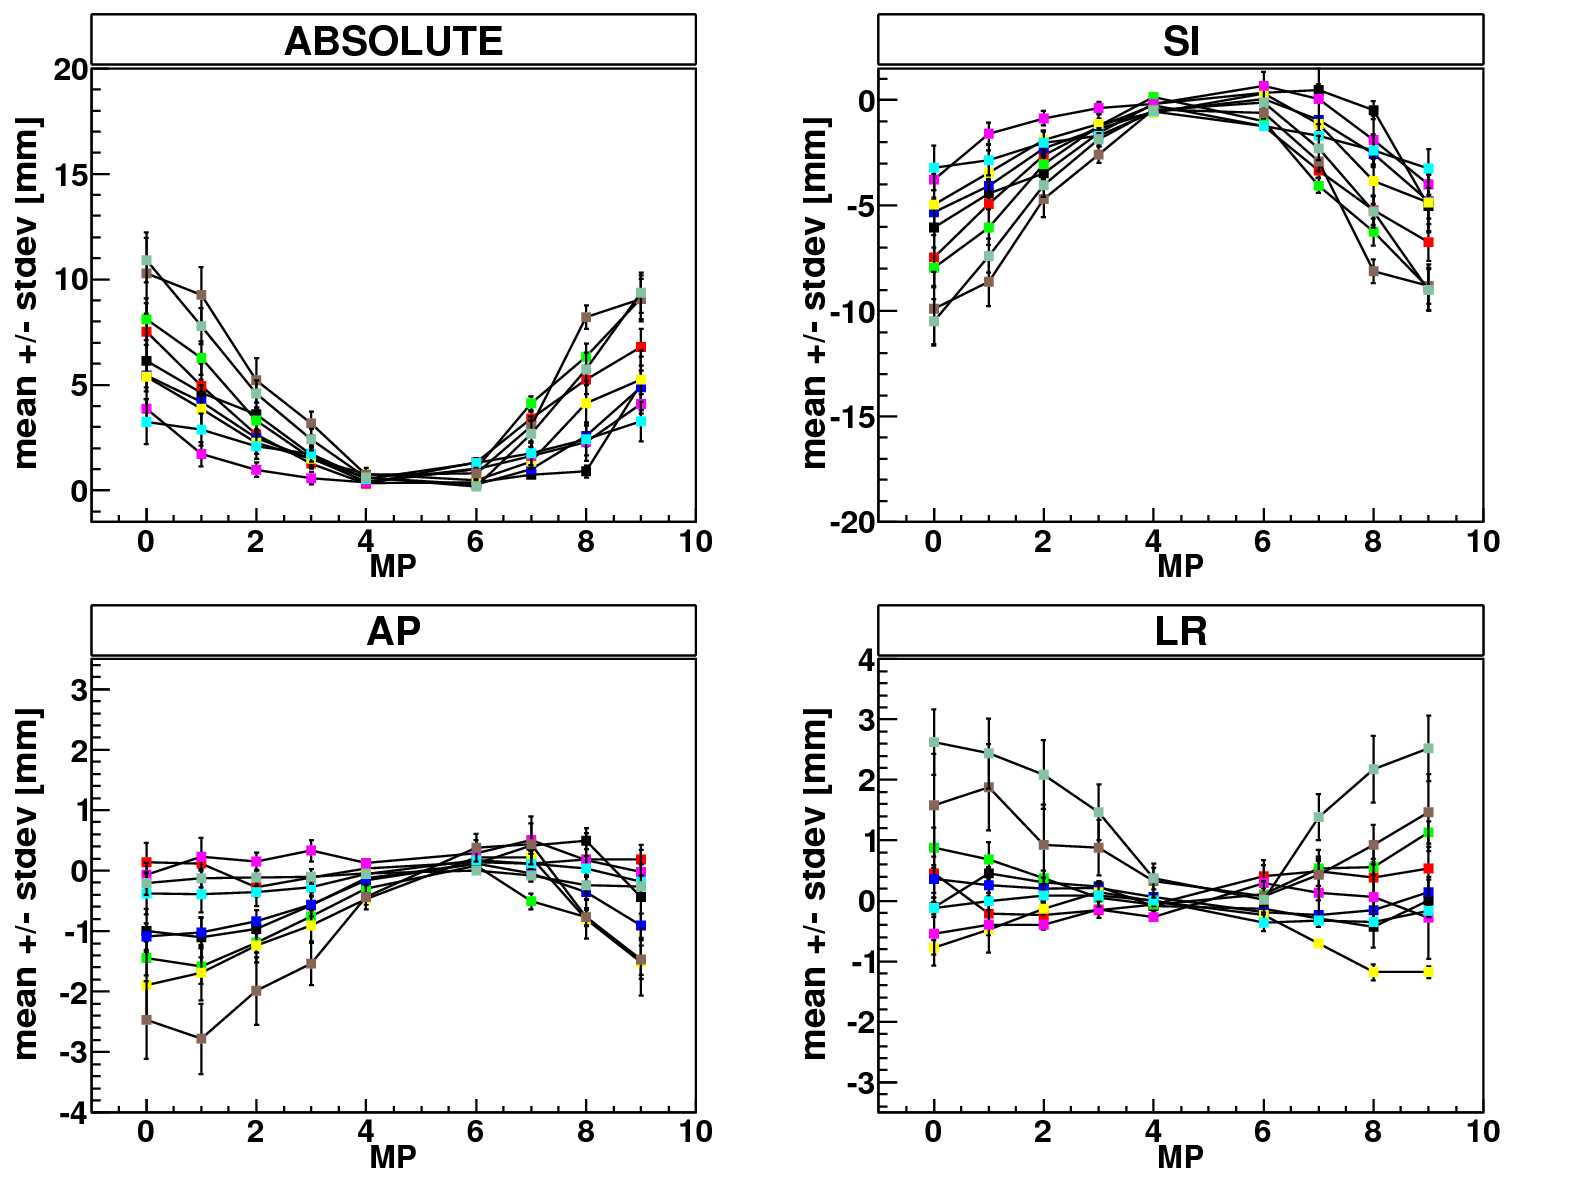
\includegraphics[scale=0.22]{./teile/results_mdacc/MDACC_allPatients_RESP_RPV.png}
\caption{RPV: Mean motion amplitude and standard deviation in each motion phase (MP) relative to the reference phase under influence of 
respiration for all patients (patient 1: black, patient 2: red, patient 3: green, patient 4: blue, patient 5: yellow, patient 6: pink, patient 
7: turquois, patient 8: brown, patient 9: olive). }
\label{motion_resp_all_rpv}
\end{center}
\end{figure}

\newpage

\begin{table}[htbp]
  \centering
  \caption{LPV: Mean and standard deviation of target motion in-between end exhale (motion phase five) and inhale (motion phase zero) for 
  all investigated patients.}
  \begin{tabular}{|c|c|c|c|c|}
    \hline\hline
    patient no & ABS [mm] & SI [mm] & AP [mm] & LR [mm]\\
    \hline
    1 & 5.2 $\pm$ 0.5 & -5.2 $\pm$ 0.5 & -0.1 $\pm$ 0.2 & -0.1 $\pm$ 0.2 \\
    2 & 5.3 $\pm$ 0.6 & -5.3 $\pm$ 0.6 & -0.4 $\pm$ 0.2 & -0.5 $\pm$ 0.2 \\
    3 & 7.1 $\pm$ 0.9 & -7.1 $\pm$ 0.9 & -0.4 $\pm$ 0.4 & -0.5 $\pm$ 0.4 \\
    4 & 3.0 $\pm$ 0.4 & -1.5 $\pm$ 0.3 & -1.9 $\pm$ 0.3 & -1.8 $\pm$ 0.5 \\
    5 & 5.1 $\pm$ 0.6 & -4.6 $\pm$ 0.5 & -0.8 $\pm$ 0.2 & -2.1 $\pm$ 0.3 \\
    6 & 6.1 $\pm$ 0.6 & -5.4 $\pm$ 0.7 & -1.4 $\pm$ 0.2 & -2.3 $\pm$ 0.2 \\
    7 & 3.9 $\pm$ 0.8 & -3.6 $\pm$ 0.6 & -1.0 $\pm$ 0.4 & -1.1 $\pm$ 0.2 \\
    8 & 9.6 $\pm$ 0.9 & -9.5 $\pm$ 0.9 & -1.0 $\pm$ 0.5 & 0.5 $\pm$ 0.4 \\
    9 & 15.5 $\pm$ 3.0 & -15.4 $\pm$ 3.0 & -0.4 $\pm$ 0.5 & -0.4 $\pm$ 1.0 \\
    \hline\hline
  \end{tabular}
  \label{tab:motion:LPV:mdacc}
\end{table}

\vspace*{-0.5cm}

\begin{table}[htbp]
  \centering
  \caption{RPV: Mean and standard deviation of target motion in-between end exhale (motion phase five) and inhale (motion phase zero) for all 
  investigated patients.}
  \begin{tabular}{|c|c|c|c|c|}
    \hline\hline
    patient no\rule{0pt}{2.6ex}\rule[-1.2ex]{0pt}{0pt} & ABS [mm] & SI [mm] & AP [mm] & LR [mm]\\
    \hline
    1 & 6.1 $\pm$ 1.4 & -6.0 $\pm$ 1.4 & -1.00 $\pm$ 0.4 & -0.1 $\pm$ 0.2 \\
    2 & 7.5 $\pm$ 1.4 & -7.5 $\pm$ 1.4 & 0.1 $\pm$ 0.3 & 0.5 $\pm$ 0.4 \\
    3 & 8.1 $\pm$ 1.0 & -7.9 $\pm$ 1.0 & -1.5 $\pm$ 0.4 & 0.9 $\pm$ 0.3 \\
    4 & 5.5 $\pm$ 0.6 & -5.3 $\pm$ 0.6 & -1.1 $\pm$ 0.2 & 0.4 $\pm$ 0.2 \\
    5 & 5.4 $\pm$ 1.5 & -5.0 $\pm$ 1.4 & -1.9 $\pm$ 0.6 & -0.8 $\pm$ 0.1 \\
    6 & 3.9 $\pm$ 0.5 & -3.8 $\pm$ 0.5 & -0.1 $\pm$ 0.2 & -0.6 $\pm$ 0.5 \\
    7 & 3.3 $\pm$ 1.1 & -3.2 $\pm$ 1.1 & -0.4 $\pm$ 0.3 & -0.1 $\pm$ 0.1 \\
    8 & 10.3 $\pm$ 1.9 & -9.9 $\pm$ 1.7 & -2.5 $\pm$ 0.6 & 1.6 $\pm$ 0.9 \\
    9 & 10.9 $\pm$ 1.1 & -10.5 $\pm$ 1.1 & -0.2 $\pm$ 0.2 & 2.6 $\pm$ 0.5 \\
    \hline\hline
  \end{tabular}
  \label{tab:motion:RPV:mdacc}
\end{table}

\vspace*{-0.5cm}

Possible correlations between the underlying respiration amplitude (see table \ref{tab:patdata}) and the displacement of the ablation sites 
for the PVs have been studied. It can be stated that in AP and LR direction, no correlation was observed. In case of SI displacement the 
results varied depending on the target volume. While no correlation was observed between the diaphragma motion and the SI displacement of the 
LPV ablation, the site for RPV showed a strong linear relationship (r=0.73, p<0.05). This resulted in a strong correlation between  
diaphragm motion and the absolute displacement of the RPV ablation site (r=0.79, p<0.05). For the LPV again no correlation was observed in the 
absolute displacement. \newline
\newline
It should be noted that these findings are based on a small number of lung cancer patients (see table \ref{tab:patdata}), which can alter the 
breathing pattern and heart motion and hence the result. It is unclear whether atrial fibrillation patients would display the same motion 
dependence and correlation results, though the result was independent of the tumor position in the left or right lung. 
\newpage
The overall displacement field between the two extreme states, end exhale and end inhale, for two exemplary patients with a small motion 
amplitude (patient 7) and a large motion amplitude (patient 9) are shown in figure \ref{contour_pat036} and \ref{contour_pat122}. In order to 
visualize the location of the displacement, an axial cut of the reference state CT is underlayed. The absolute values of the displacement 
vectors are shown as contour plots. 

\begin{figure}[H]
\begin{center}
 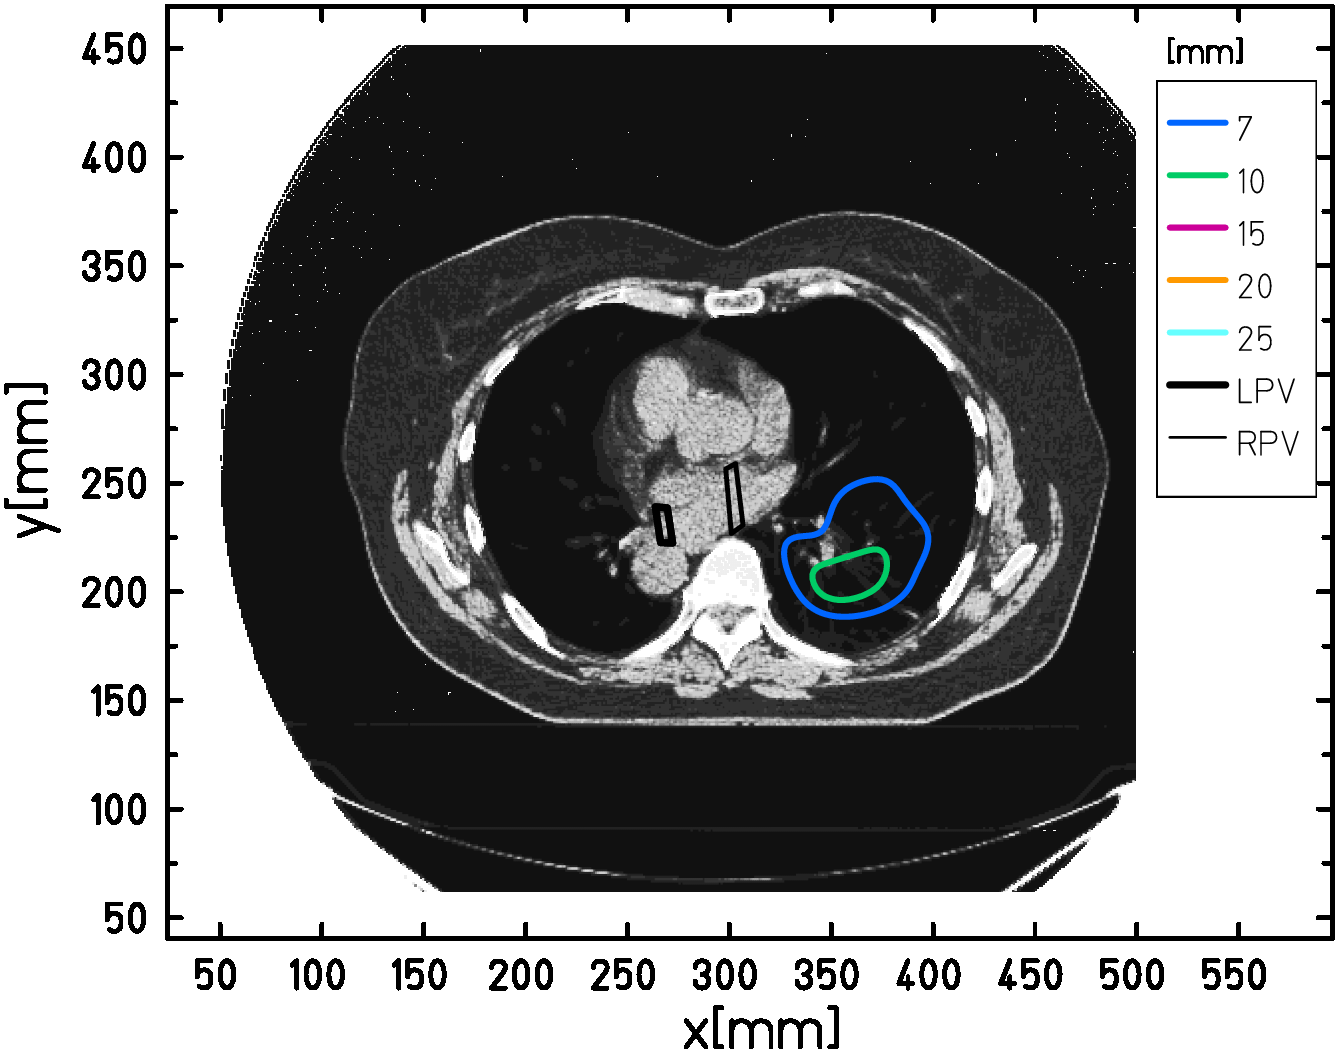
\includegraphics[scale=0.22]{./teile/results_mdacc/Contour_z_abs_RESP_Pat037_HUSkala_gedreht_2.png}
\caption{Contour plot of Patient 7}
\label{contour_pat036}
\end{center}
\end{figure}

\vspace*{-0.3cm}

\begin{figure}[H]
\begin{center}
 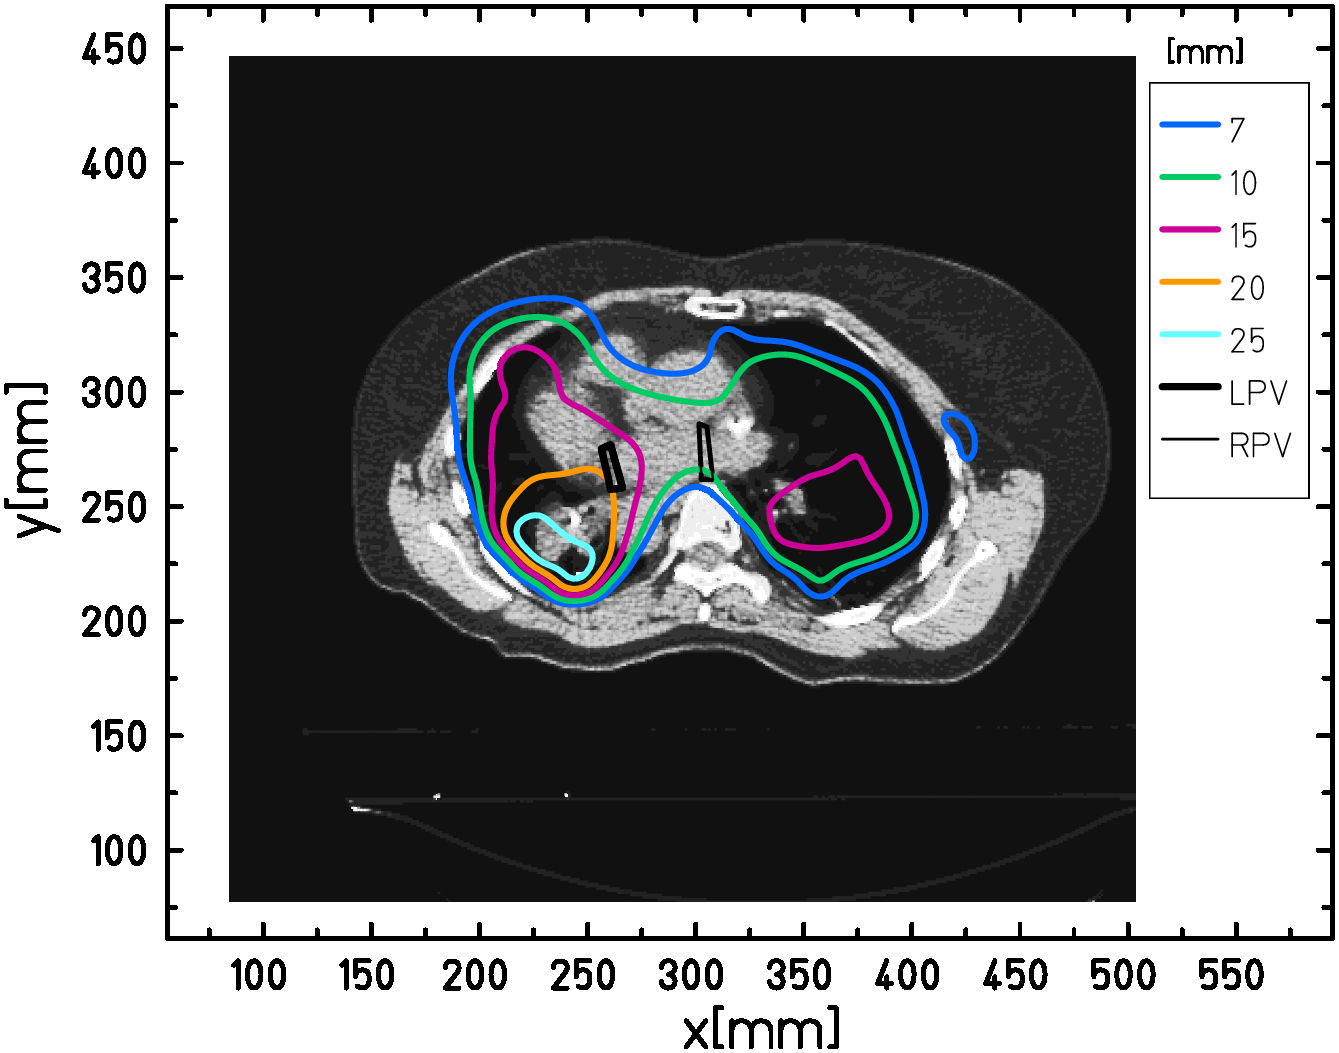
\includegraphics[scale=0.22]{./teile/results_mdacc/Contour_z_abs_RESP_Pat122_HUSkala_gedreht_2.png}
\caption{Contour plot of Patient 9 }
\label{contour_pat122}
\end{center}
\end{figure}

\newpage


\subsection{Motion mitigation techniques for respiration}
\label{mmt}
The absolute motion amplitudes of up to 1cm due to respiration are expected to yield dose inhomogeneity when not compensated for. The 
resulting interplay effect and dose deposition were studied for every patient for different motion patterns and different margins to the target 
volumes. The dose analysis values V95, V107 and D5-D95 were assessed and plotted. For comparison also the corresponding 
values for the 3D case (static) are shown. As shown in section \ref{motion} the motion displacement in the motion phases around 
end exhale (motion phase four to motion phase six) are rather small in all patient cases. Hence gating has the potential to be a 
well-suited motion mitigation technique to overcome the influence of target volume motion due to respiration. The results of the stated dose 
values in case of gating on the stated phases will be presented. 


\subsubsection{Dose deposition}

A representative dose deposition for all studied techniques (static, interplay and gating) is shown exemplary for patient 9 (as this is the 
patient with the largest PV motion amplitude) in figure \ref{dose_pat122}. Gating and interplay are shown for a motion period of 6s 
and a starting phase of 0$^{\circ}$. The target volumes LPV and RPV were irradiated simultaneously and a margin of 3mm was added. It can 
already been seen from these dose cut figures that gating around end expiration drastically improves the outcome compared to interplay and yields 
a result which is comparable to the static case.\newline
\newline
In order to assess the dose information for the whole volume the DVHs (see figure \ref{dvhs_pat09_mdacc}) of all patients were analyzed and compared for dose homogeneity, 
dose coverage as well as over dosage. The average results over all patients with the resulting standard deviation can be seen in 
figure \ref{static_interplay_gating}. A more detailed analysis can be found in appendix \ref{app:mdacc}, where the corresponding numerical 
values are shown (tables \ref{tab:Pat01:LPV} - \ref{tab:Pat09:RPV}) .\newline
\newline
For interplay it can be seen that the results are dependent on the used motion period and starting phase. This can be seen in the 
mean values of the resulting dose parameter values for different underlying motion patterns. E.g. for LPV, the mean value of the dose 
coverage parameter over all patients is V95=(90.3 $\pm$ 4.3)\% for a motion with 6s period and a starting phase of 90$^{\circ}$ and 
(89.3 $\pm$ 5.5)\% for a motion period of 8s and starting phase of 90$^{\circ}$, while for a motion period of 8s 
and a starting phase of 0$^{\circ}$ the dose coverage is (87.1 $\pm$ 7.8)\%. 
The safety margin influences the treatment outcome, as e.g. the dose coverage for a motion with 6s period 
and a starting phase of 90$^{\circ}$ has a mean value of (94.2 $\pm$ 4.8)\% with 3mm safety margin. All these dependencies are also valid for 
the other studied dose analysis parameters, dose homogeneity and over dosage. The improvement of the dose coverage and dose homogeneity 
in relation to the size of the safety margin are also presented in figure \ref{static_interplay_gating_ALLpatients_KORR} (a and b). 
The explained variance of the dose homogeneity versus the studied safety margins resulted in $r^{2}$=0.30 (p<0.0001).\newline 
\newline
The underlying deformation map with its motion amplitude enables a prediction of the magnitude of the interplay effect. 
This was studied in more detail for the dose homogeneity, as these values were normally distributed. 
The explained variance of the maximal motion amplitude of the left and right PV (see table \ref{tab:motion:LPV:mdacc} and 
\ref{tab:motion:RPV:mdacc}) and the resulting D5-D95 values for all studied margins was $r^{2}$=0.25 (p<0.0001).\newline 
\newline
Gating yielded improved results compared to interplay in all studied cases (see also figure \ref{static_interplay_gating_ALLpatients_KORR}). 
This is valid for dose homogeneity, dose coverage as 
well as over dosage. Especially dose coverage and over dosage are comparable to the static results for all patient and motion patterns 
(e.g. patient 1, V95 of 100\% for all studied motion patterns and safety margins in RPV, see table \ref{tab:Pat01:RPV}). In some patients the 
dose coverage is better with added safety margins (e.g. patient 9, V95 with no margin for motion period of 6s and starting phase of 0$^{\circ}$ is 94.1\% for LPV, 
a V95 of 99.9\% can be achieved for the same motion pattern with a margin of 3mm). Also in dose homogeneity a bigger safety margin tends to 
improve results (e.g. in LPV of patient 1 with motion period of 8s with starting phase of 0$^{\circ}$: D5-D95 = 4.4\% with margin of 3mm 
versus D5-D95 = 3.8\% with margin of 5mm). These findings are also shown in figure \ref{static_interplay_gating_ALLpatients_KORR}. Here 
the dose coverage and dose homogeneity are shown for all patients, motion patterns and the two target sites (LPV and RPV) depending on the 
used safety margin. It can be seen that the dose coverage is already drastically improved with 3mm margin. Also the dose homogeneity is 
improved with increasing safety margin. 
The explained variance of D5-D95 versus all studied margins resulted in $r^{2}$=0.40 (p<0.0001). 
Keeping the safety margin constant, it was nevertheless found that in some cases 
the dose homogeneity is not drastically improved by gating compared to interplay. The LPV of patient 2 for example 
has a D5-D95 value of 6.8\% for gating with a safety margin of 3mm (motion period of 6s and starting phase of 90$^{\circ}$), which is 
only slightly under the interplay result of D5-D95=8.4\% for the same safety margin and motion. However, the dose homogeneity value of 
interplay in this particular patient case is already lower than in other cases (e.g. D5-D95=10.6\% in patient 1 or 20.93\% in patient 9 
for 3mm margin and a motion period of 6s, starting phase of 90$^{\circ}$).\newline
\newline
As a method to further improve the dose homogeneity rescanning inside the gating window was studied for two patient cases. The results are 
presented in the next section. It can nevertheless be concluded that gating of target volumes with safety margin yields results comparable to 
the static irradiation in case of under and overdosage and hence is an adequate motion mitigation technique for the irradition of the 
PVs under influence of respiration. 



\newpage

 \begin{figure}[H]
 \begin{center}
\subfigure[static]{
 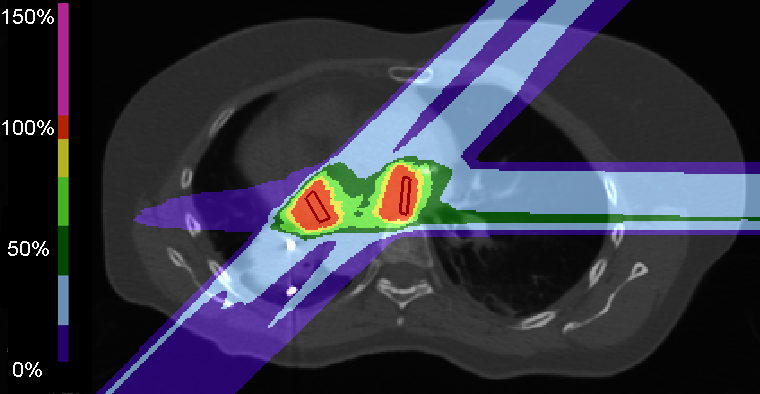
\includegraphics[scale=0.6]{./teile/results_mdacc/Pat122_slice50_static.png}
 }
\subfigure[interplay]{
 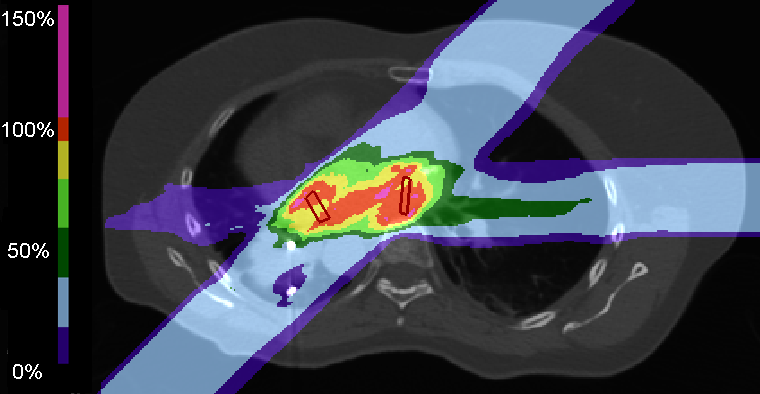
\includegraphics[scale=0.6]{./teile/results_mdacc/Pat122_slice50_interplay.png}
 }
 \subfigure[gating]{
 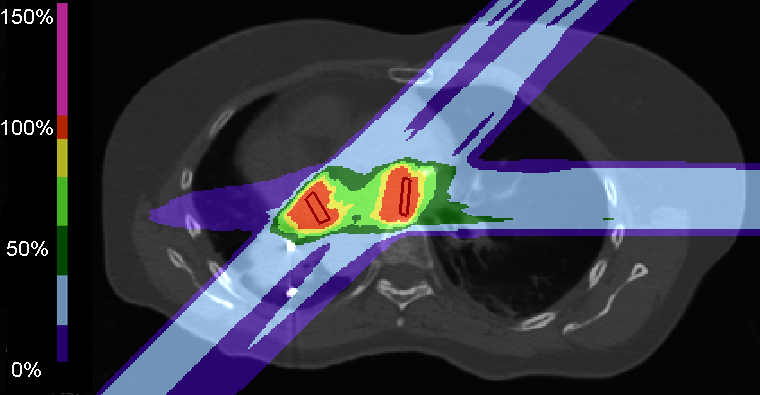
\includegraphics[scale=0.6]{./teile/results_mdacc/Pat122_slice50_gating.png}
 }
\caption{Dose distribution of patient 9 for static (a) as well as interplay (b) and gating (c) at motion period of 6s and a motion starting 
phase of 0$^{\circ}$. The target volume has an added margin of 3mm. The improved outcome of gating compared to interplay 
can already be seen in these dose cuts.}
\label{dose_pat122}
 \end{center}
\end{figure}

\newpage


 \begin{figure}[H]
 \begin{center}
\subfigure[LPV]{
 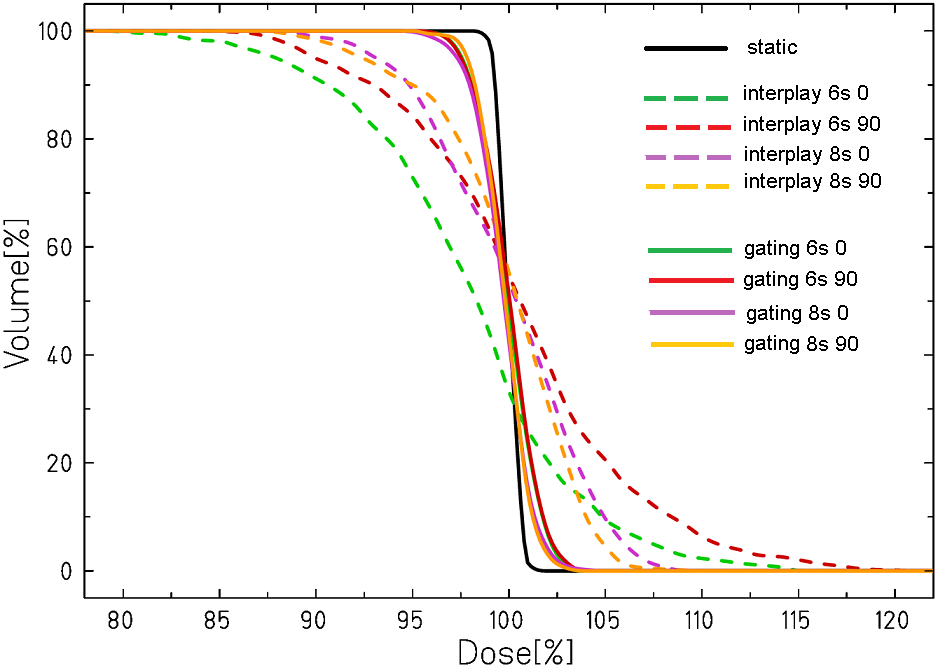
\includegraphics[scale=0.48]{./teile/results_mdacc/Pat09_allDVHs_LPV_withLegend.png}
 }
\subfigure[RPV]{
 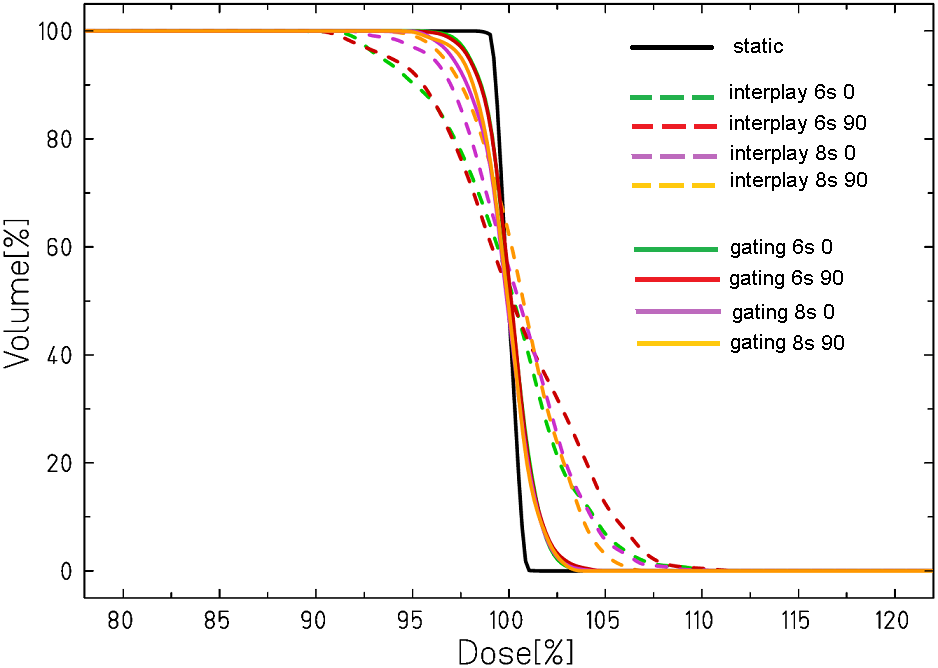
\includegraphics[scale=0.48]{./teile/results_mdacc/Pat09_allDVHs_RPV_withLegend.png}
 }
\caption{Dose volume histograms for CTV of patient 9 for 3mm safety margin irradiation (LPV (a) as well as RPV (b)) in case of static 
irradiation (black), interplay (dashed) and gating (solid). The motion patterns are shown in colors (6s 0: lujan motion with period of 6s 
and starting phase 0$^{\circ}$, 6s 90: lujan motion period of 6s and starting phase 90$^{\circ}$, 8s 0: lujan motion period of 8s 
and starting phase 0$^{\circ}$, 8s 90: lujan motion period of 8s and starting phase 90$^{\circ}$.}
\label{dvhs_pat09_mdacc}
 \end{center}
\end{figure}

\newpage

\begin{figure}[H]
\subfigure[D5-D95: LPV]{
 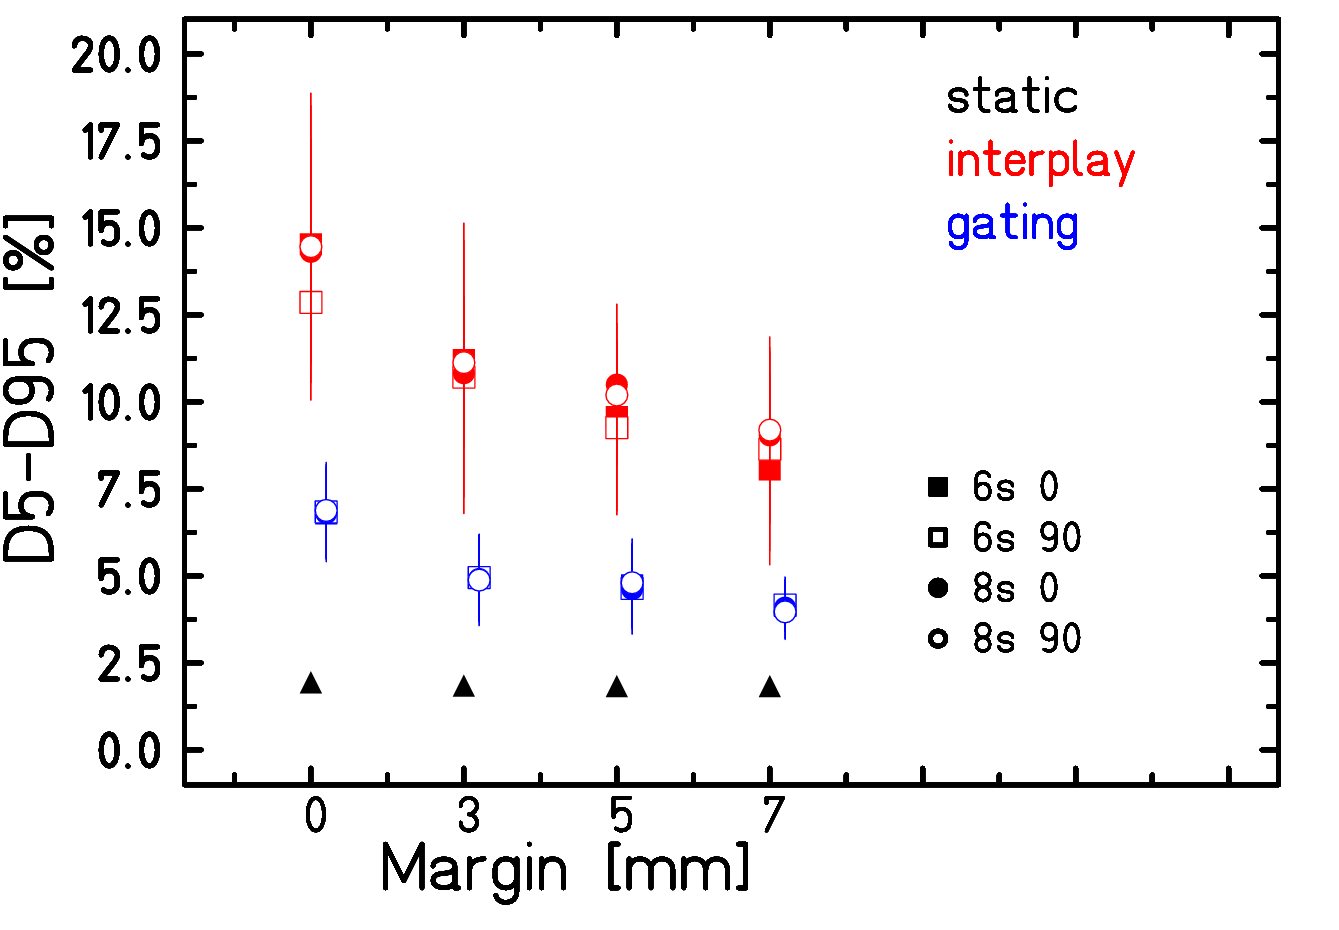
\includegraphics[scale=0.18]{./teile/results_mdacc/MDACC_CTV_LPV_D5D95.png}
 }
 \subfigure[D5-D95: RPV]{
 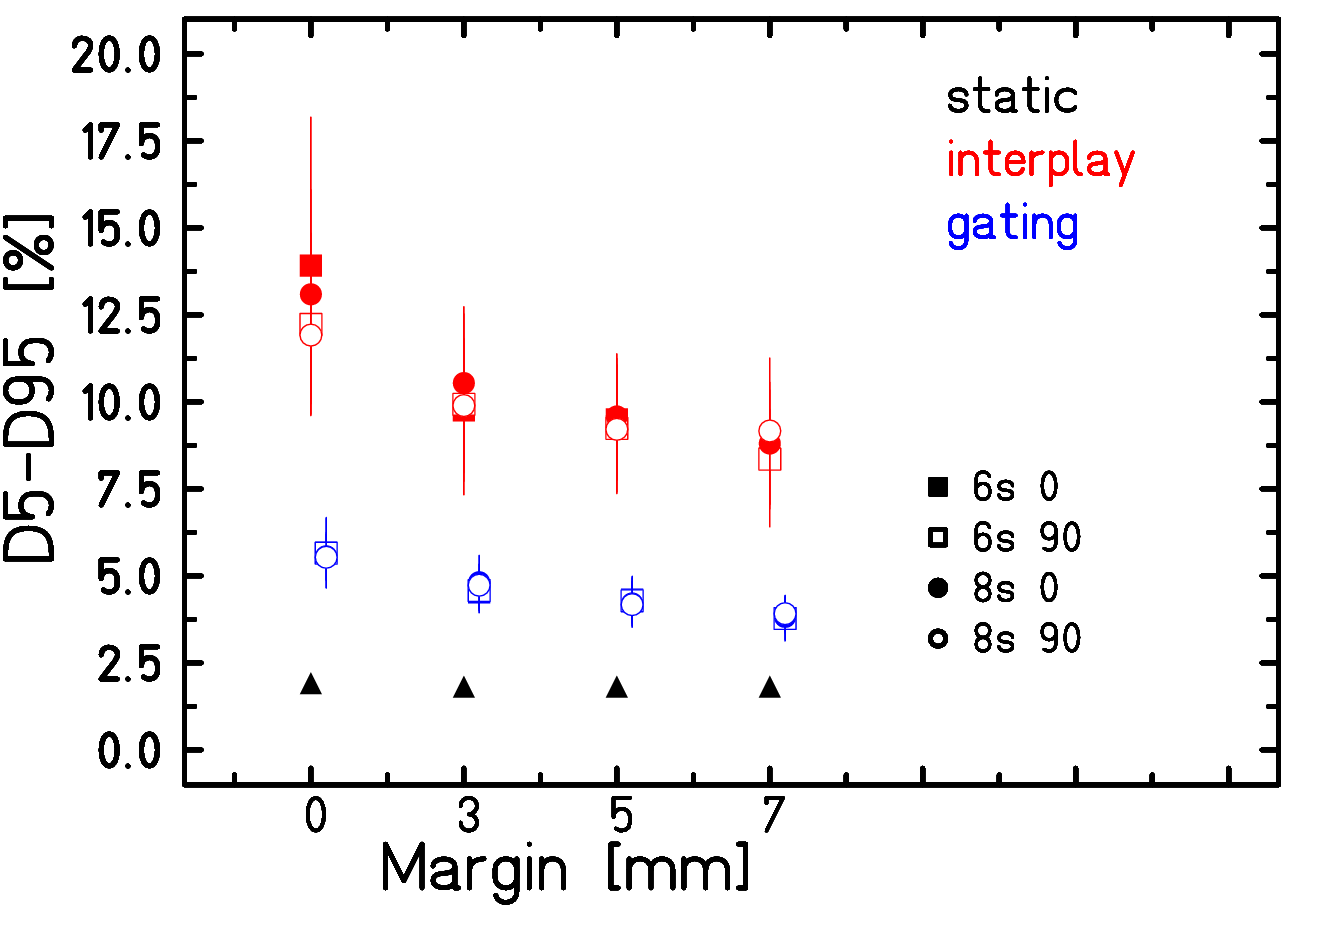
\includegraphics[scale=0.18]{./teile/results_mdacc/MDACC_CTV_RPV_D5D95.png}
 }
 \subfigure[V95: LPV]{
 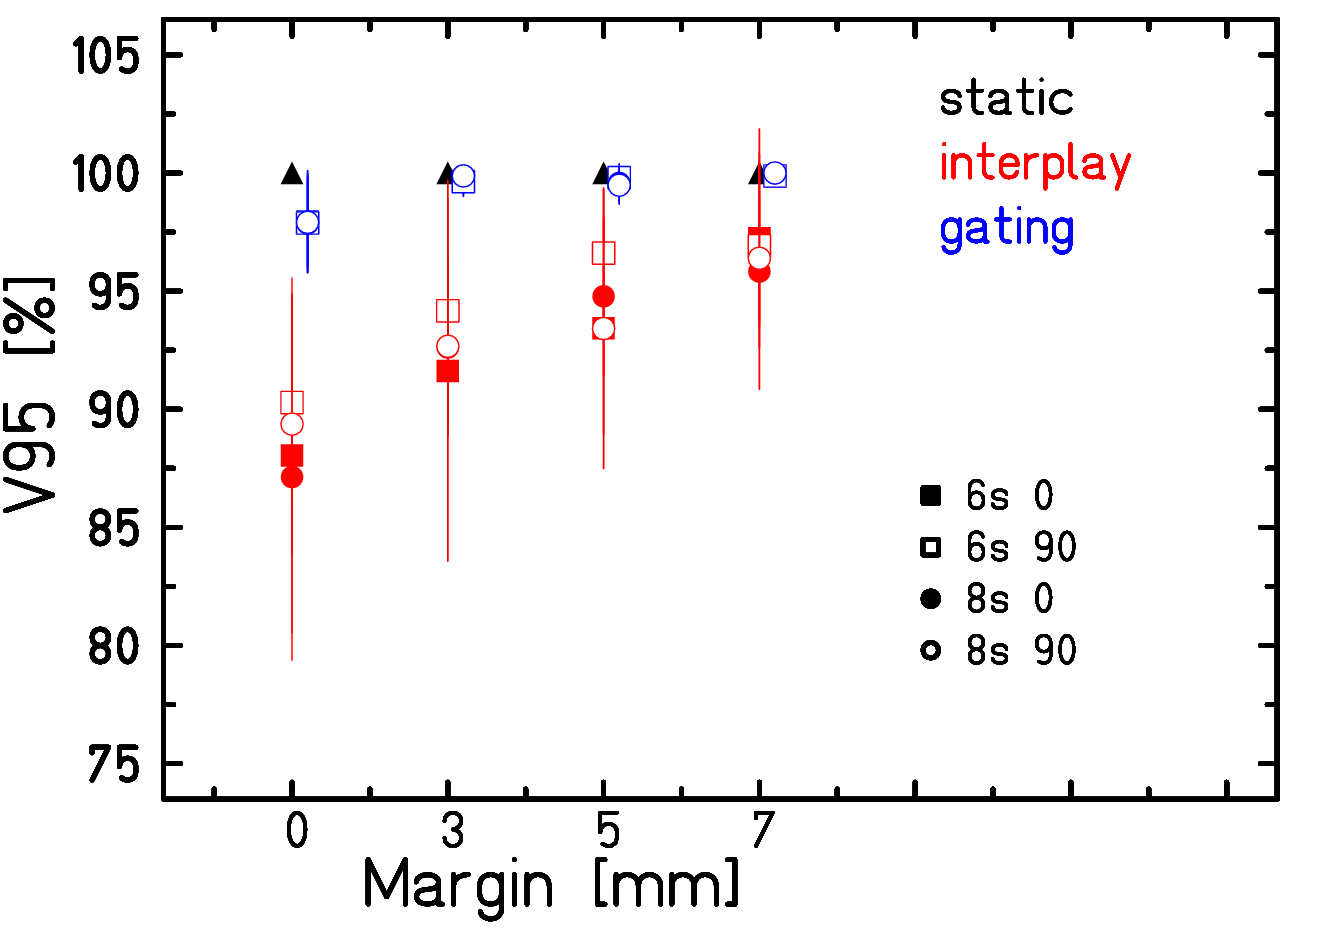
\includegraphics[scale=0.18]{./teile/results_mdacc/MDACC_CTV_LPV_V95.png}
 }
\subfigure[V95: RPV]{
 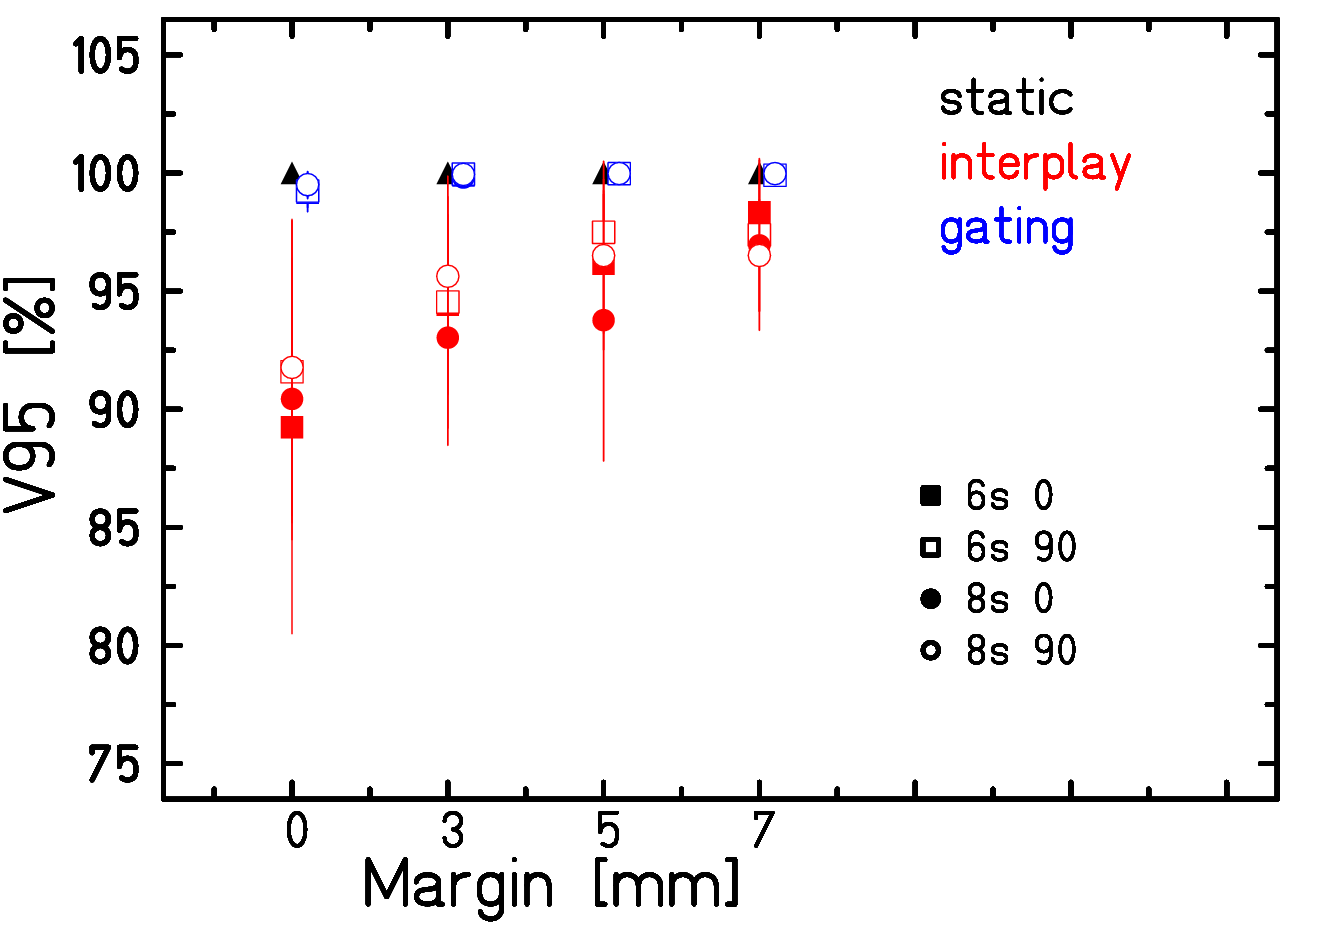
\includegraphics[scale=0.18]{./teile/results_mdacc/MDACC_CTV_RPV_V95.png}
 }
  \subfigure[V107: LPV]{
 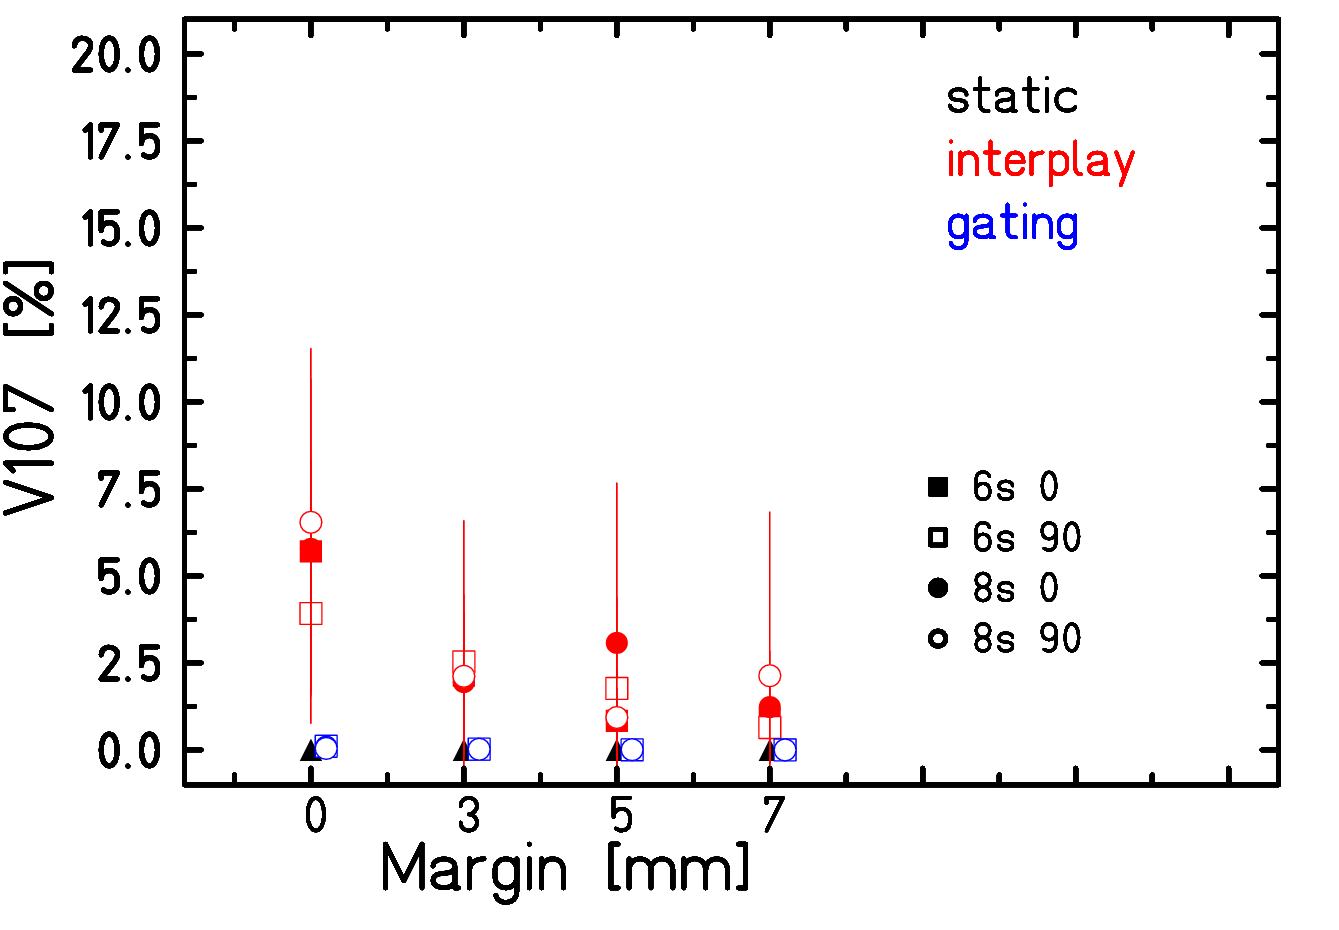
\includegraphics[scale=0.18]{./teile/results_mdacc/MDACC_CTV_LPV_V107.png}
 }
\subfigure[V107: RPV]{
 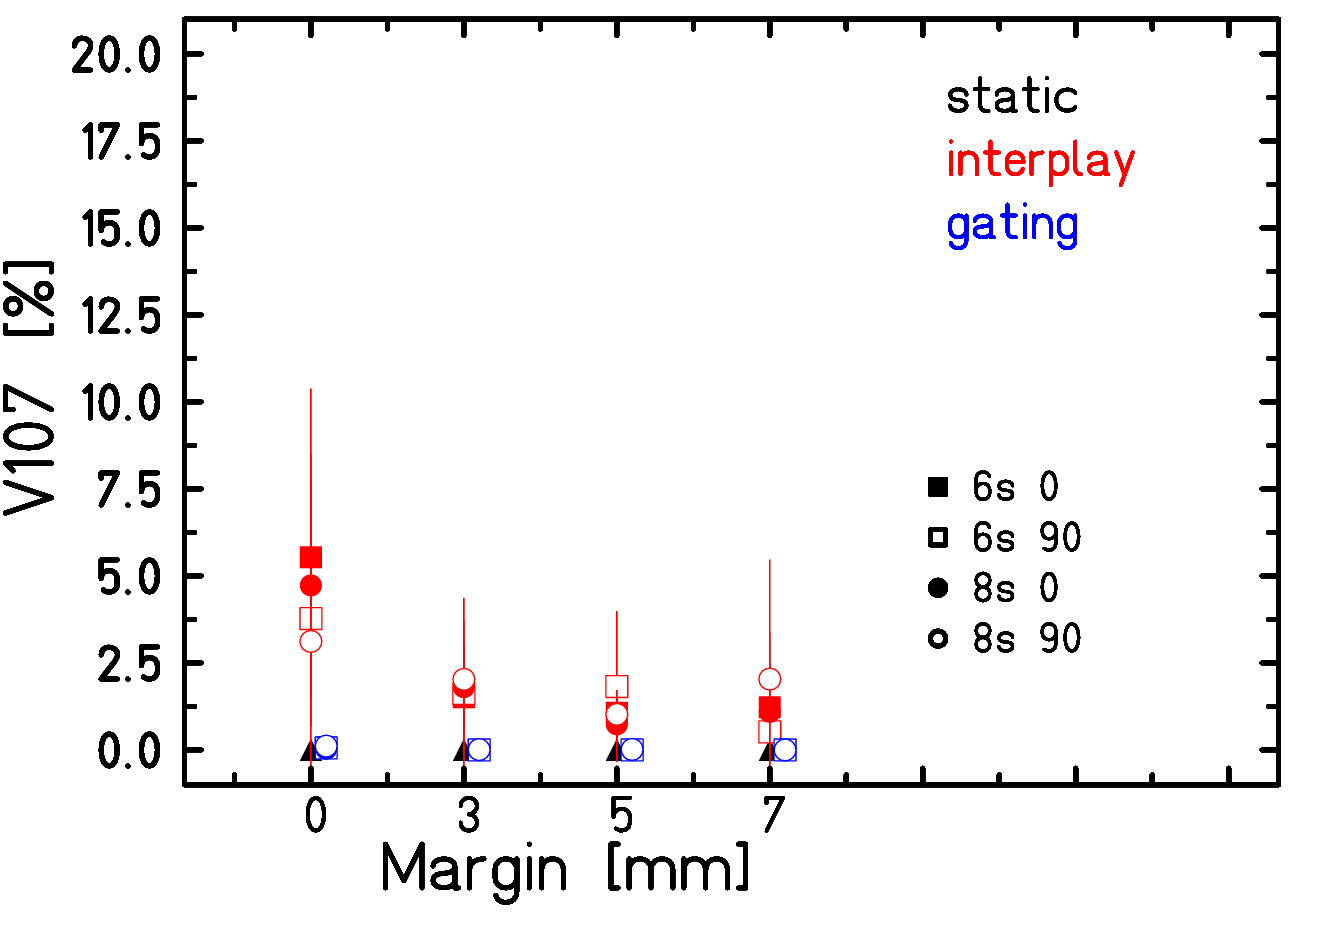
\includegraphics[scale=0.18]{./teile/results_mdacc/MDACC_CTV_RPV_V107.png}
 }
\caption{Mean value and standard deviation of dose analysis parameters D5-D95 (first row), V95 (middle row) 
and V107 (last row) over all patients. The LPV (left column) and RPV (right column) were studied seperately. Static (black) as well as interplay (red) and gating (blue) 
are compared for four different motions and different safety margins.}
\label{static_interplay_gating}
\end{figure}

\newpage 

\begin{figure}[H]
\centering
\subfigure[D5-D95 versus margin size]{
 \includegraphics[scale=0.75]{./teile/results_mdacc/D5D95_vs_margin_2.png}
 }
 \subfigure[V95 versus margin size]{
 \includegraphics[scale=0.75]{./teile/results_mdacc/V95_vs_margin_2.png}
 }
\caption{(a) and (b): Boxplot of dose analysis parameters D5-D95 and V95 over all patient data sets, motion patterns and target volumes (LPV: circle and 
RPV: cross) depending on the used margins size (0mm, 3mm, 5mm and 7mm) and irradiation mode (static, interplay and gating). Here, minimum and 
maximum of the data is plotted within 1.5 times the interquartile range, the other data points are stated as outliers. 
Figures are courtesy of Dr. Christian Graeff.}
\label{static_interplay_gating_ALLpatients_KORR}
\end{figure}

\newpage


\subsubsection*{Rescanning of gated volume}
\label{RescanofGate}

The combination of two motion mitigation techniques, gating and rescanning, would directly apply when not only the respiratory motion but 
also the heartbeat would be compensated for (see chapter \ref{chapter:human}). In order to study the outcome of such a delivery, several 
number of rescans (5, 10, 15 and 20) were applied on the gated irradiation for patient 2 (as an example of a patient with a medium absolute 
displacement of the target volumes) and patient 9 (with the highest studied absolute displacement). The results can be seen in figure 
\ref{static_interplay_gating_rescan_Pat02} and \ref{static_interplay_gating_rescan_Pat09}. For patient 9 the DVHs for static as well as 
the gating results for all motion patterns and the corresponding results for ten rescans within the gating window are shown in 
figure \ref{dvhs_pat09_mdacc_rescan}. All numerical results are shown in appendix \ref{app:mdacc} (tables \ref{tab:pat02:LPV:rescan} to 
\ref{tab:pat09:RPV:rescan}).\newline
\newline
It becomes obvious that rescanning does further improve the dose delivery regarding dose homogeneity. For patient 2 the 
dose homogeneity value of 6.8\% of the prescribed physical dose of 25Gy achieved with gating in the LPV (3 mm margin, motion period of 6s and starting 
phase of 90$^{\circ}$) can be slightly improved to 4.7\% with five rescans or 3.8\% with ten rescans. In RPV the dose homogeneity value of 
patient 2 of 5.0\% for the same margin and motion can be improved to 4.8\% with five rescans and 4.1\% with ten rescans. 
For patient 9 the dose homogeneity value of 5.0\% for LPV with 3mm margin and motion period of 6s, starting phase of 90$^{\circ}$ can 
be improved to 3.8\% with five rescans. For the RPV dose homogeneity of 4.4\% with the same margin and motion can be reduced to 
3.9\% with five rescans. Rescan numbers higher than ten only lead to a minor improvement. For example in Patient 9 the LPV irradiation with 
3mm margin and the stated motion of 6s period and 90$^{\circ}$ starting phase results in 3.7\%, both for fifteen and twenty rescans, 
respectively.\newline
\newline
It can be concluded that the dose homogeneity can be slightly improved with rescanning within the gating window. A small number of rescans, 
e.g. five or ten, are already sufficient to yield acceptable results and the outcome can not be improved by using higher rescan numbers. 
As rescanning will be studied as motion mitigation technique for the heartbeat motion influence, the overlay of rescanning and gating will be 
carried out automatically in case of an application of the here studied non-invasive treatment modality for atrial fibrillation, as both, 
respiration and heartbeat, need to be accounted for. 

\newpage

\begin{figure}[H]
\subfigure[D5-D95: LPV]{
 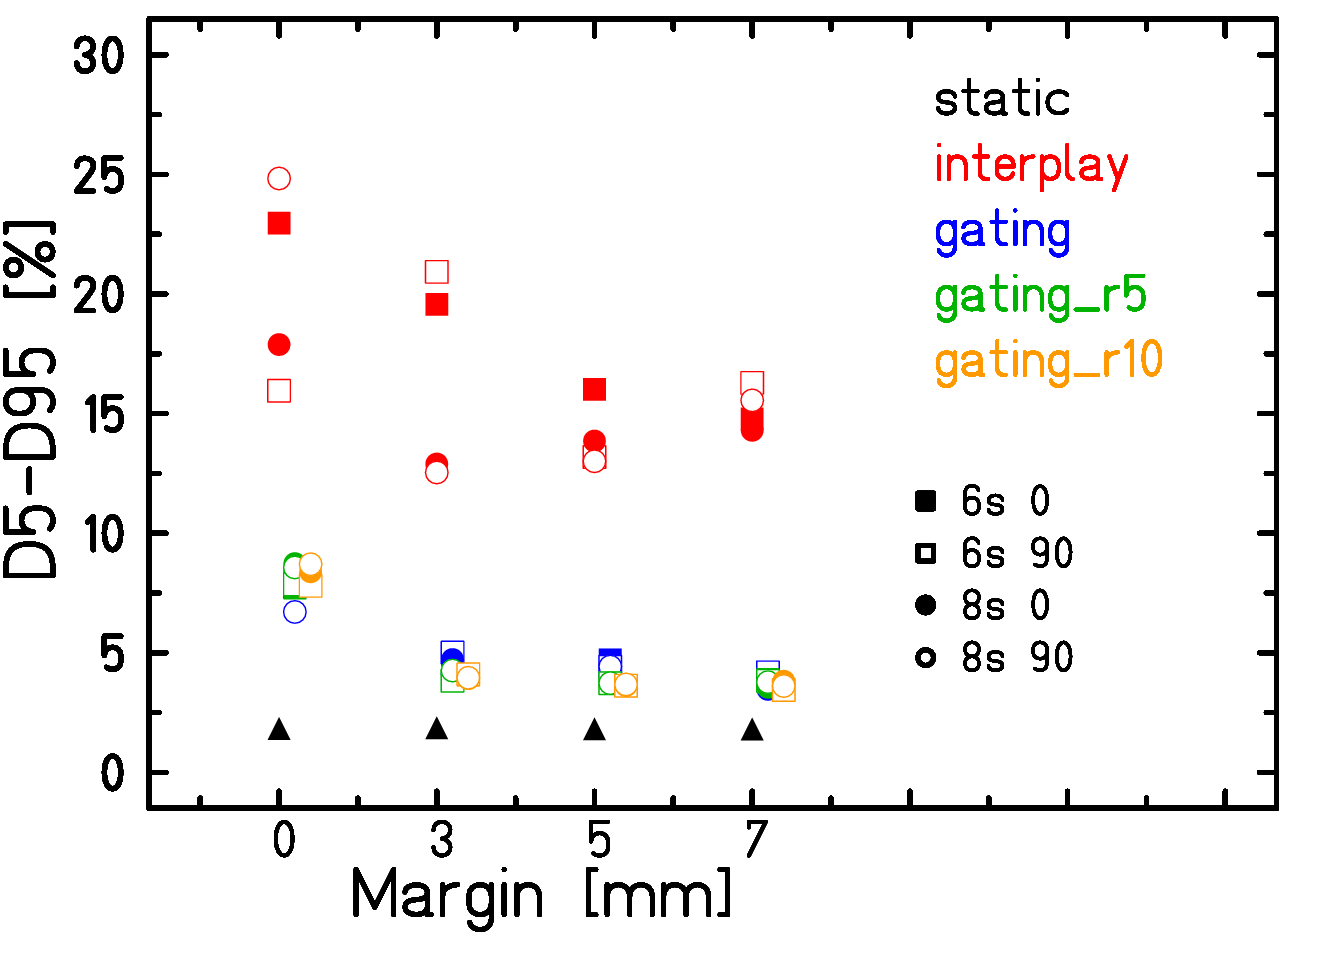
\includegraphics[scale=0.18]{./teile/results_mdacc/MDACC_Pat122_CTV_LPV_D5D95_withRescan.png}
 }
 \subfigure[D5-D95: RPV]{
 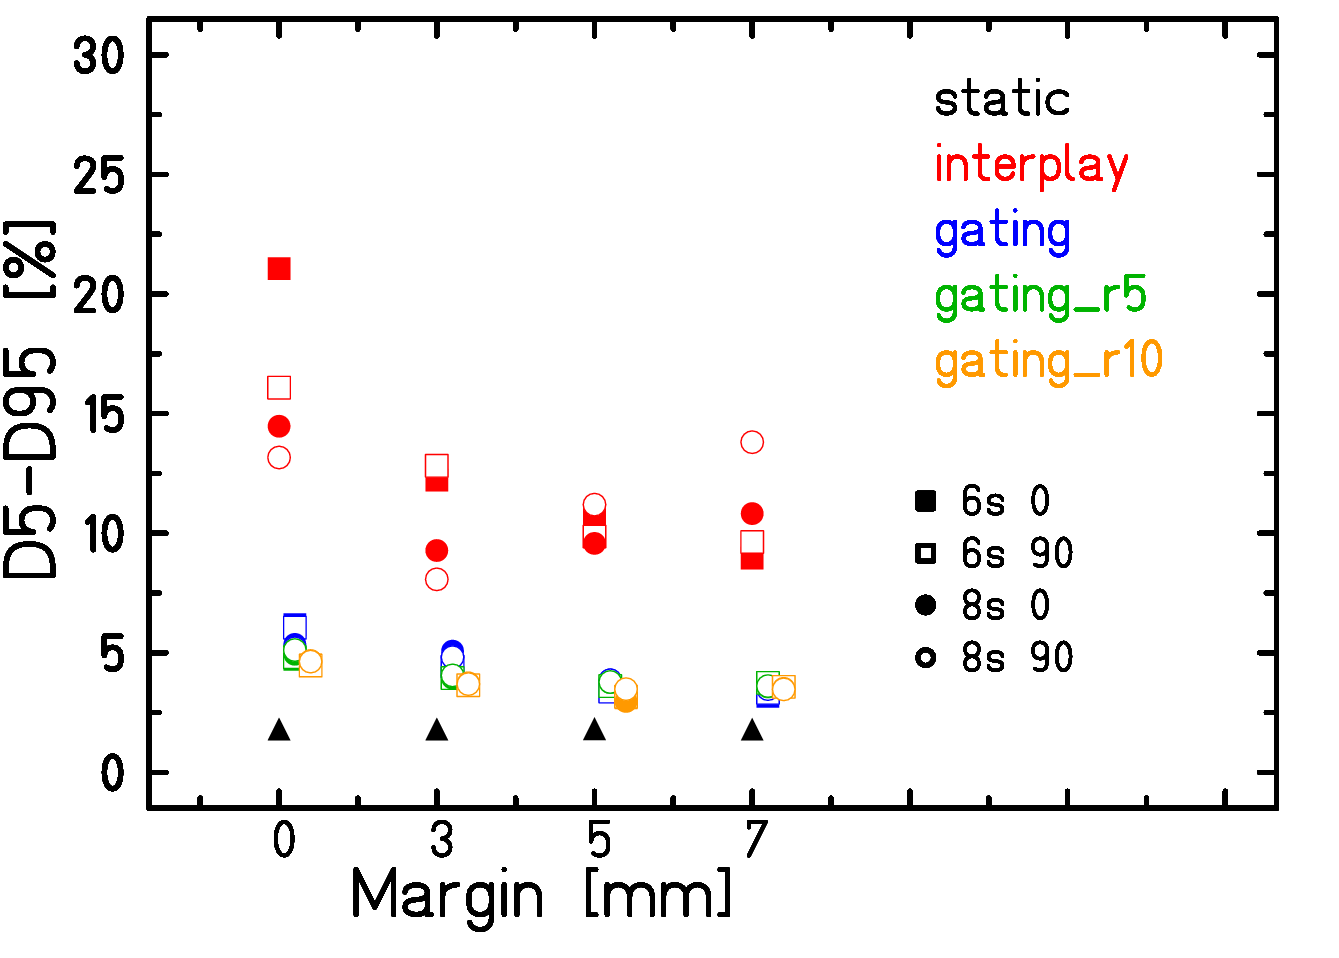
\includegraphics[scale=0.18]{./teile/results_mdacc/MDACC_Pat122_CTV_RPV_D5D95_withRescan.png}
 }
 \subfigure[V95: LPV]{
 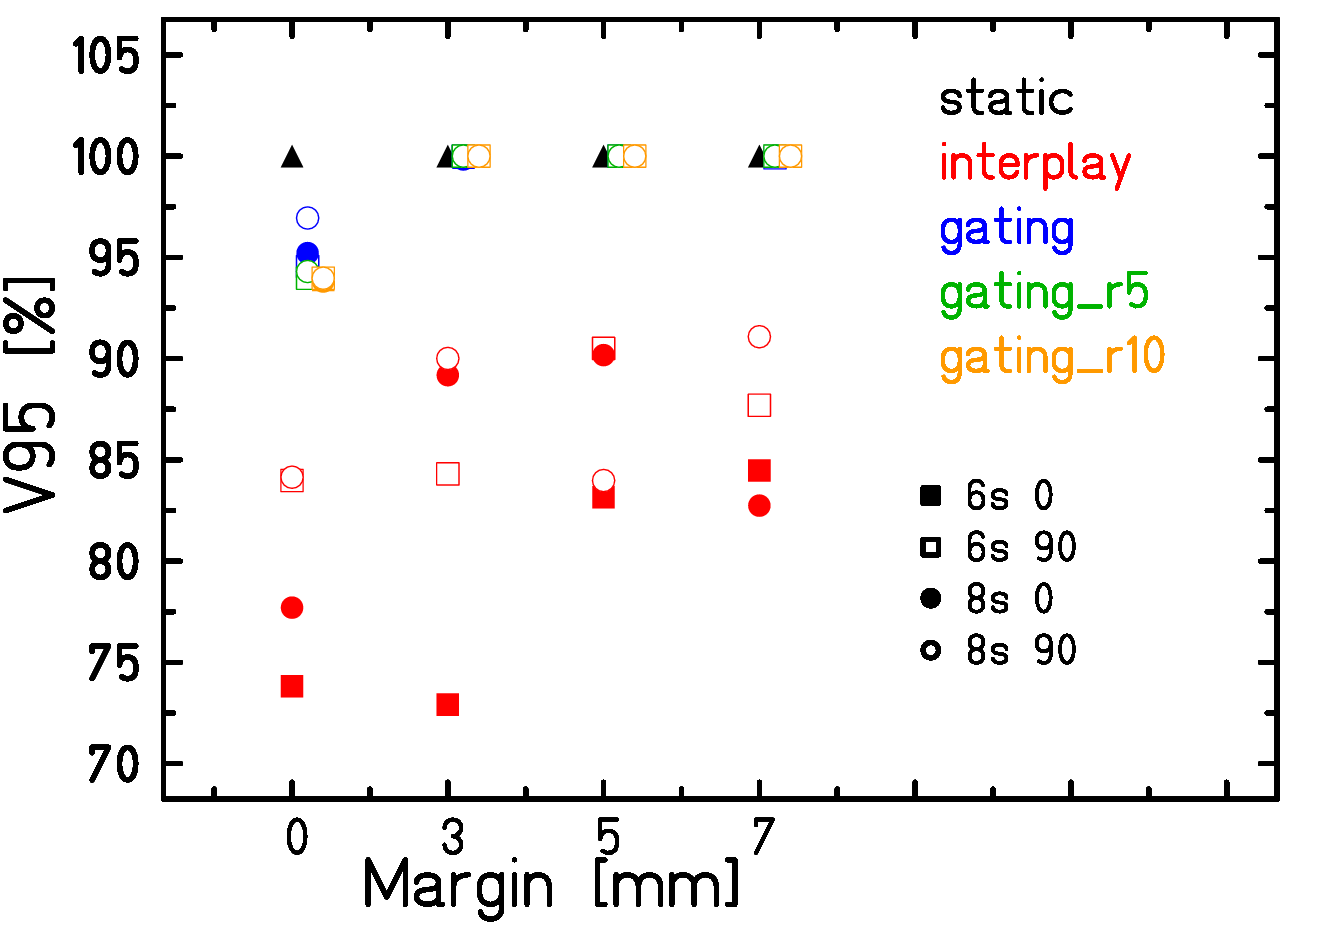
\includegraphics[scale=0.18]{./teile/results_mdacc/MDACC_Pat122_CTV_LPV_V95_withRescan.png}
 }
\subfigure[V95: RPV]{
 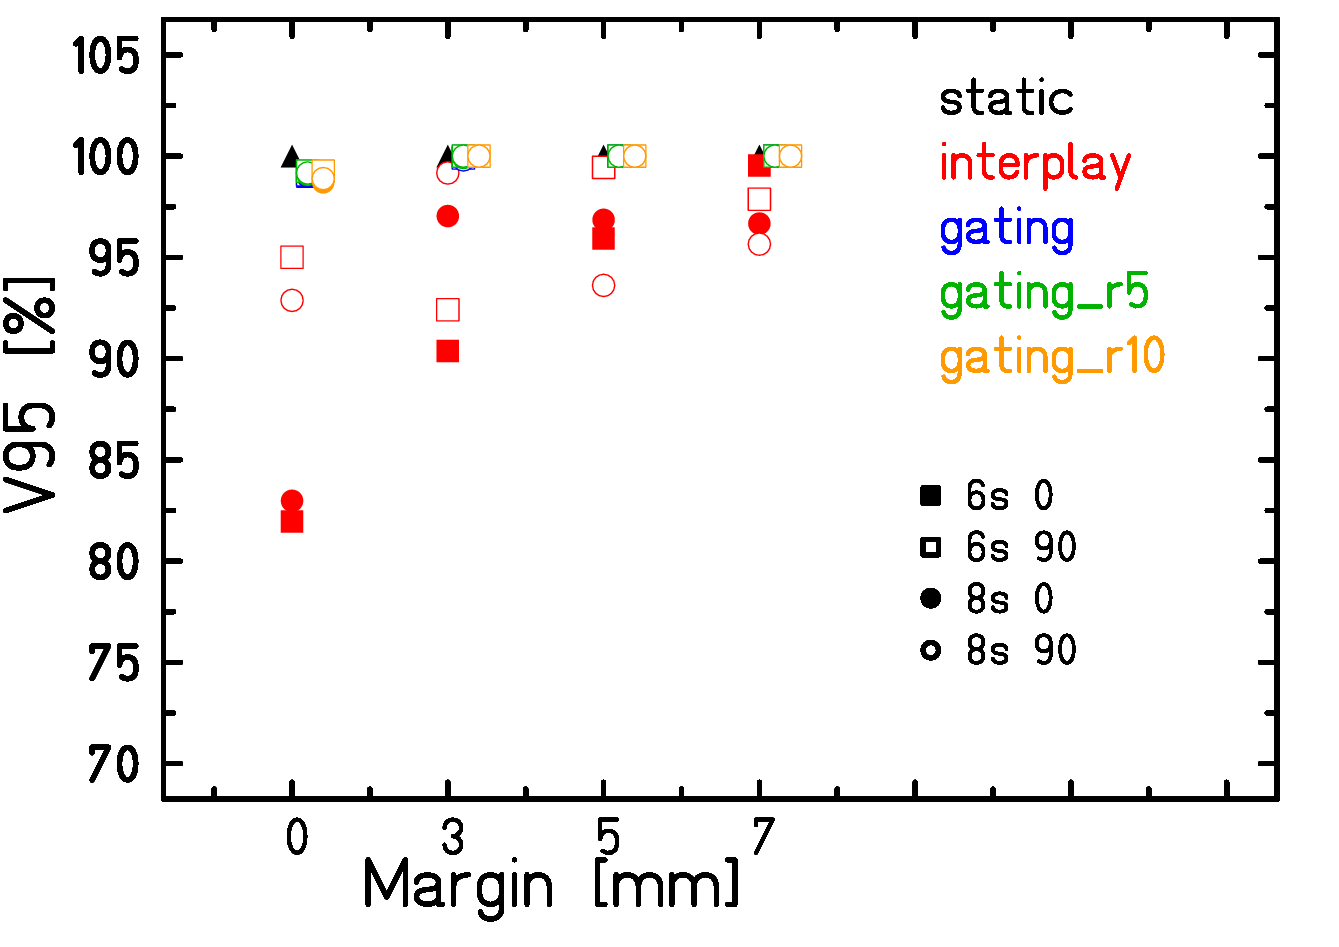
\includegraphics[scale=0.18]{./teile/results_mdacc/MDACC_Pat122_CTV_RPV_V95_withRescan.png}
 }
  \subfigure[V107: LPV]{
 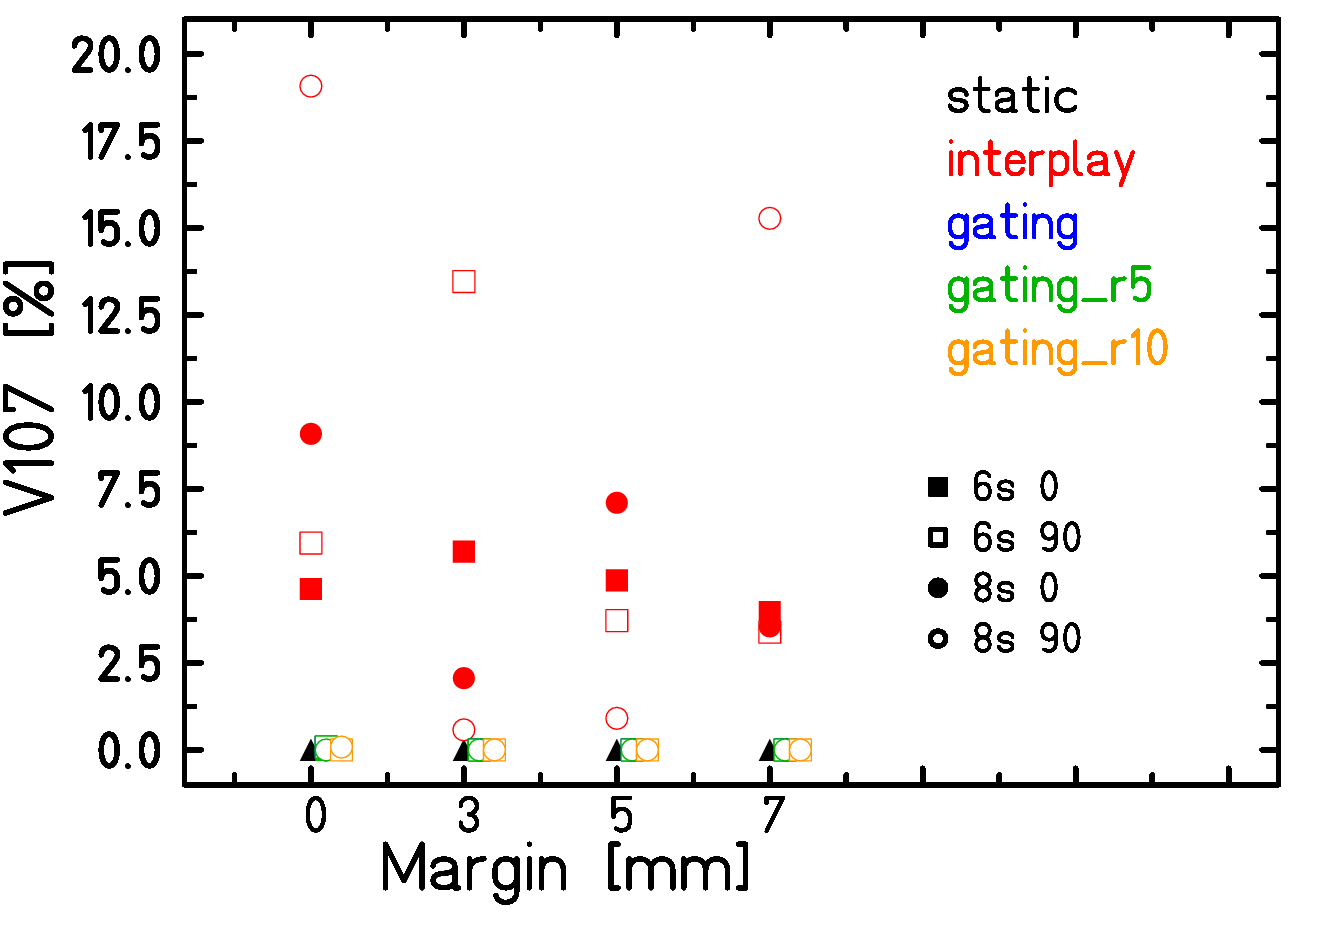
\includegraphics[scale=0.18]{./teile/results_mdacc/MDACC_Pat122_CTV_LPV_V107_withRescan.png}
 }
\subfigure[V107: RPV]{
 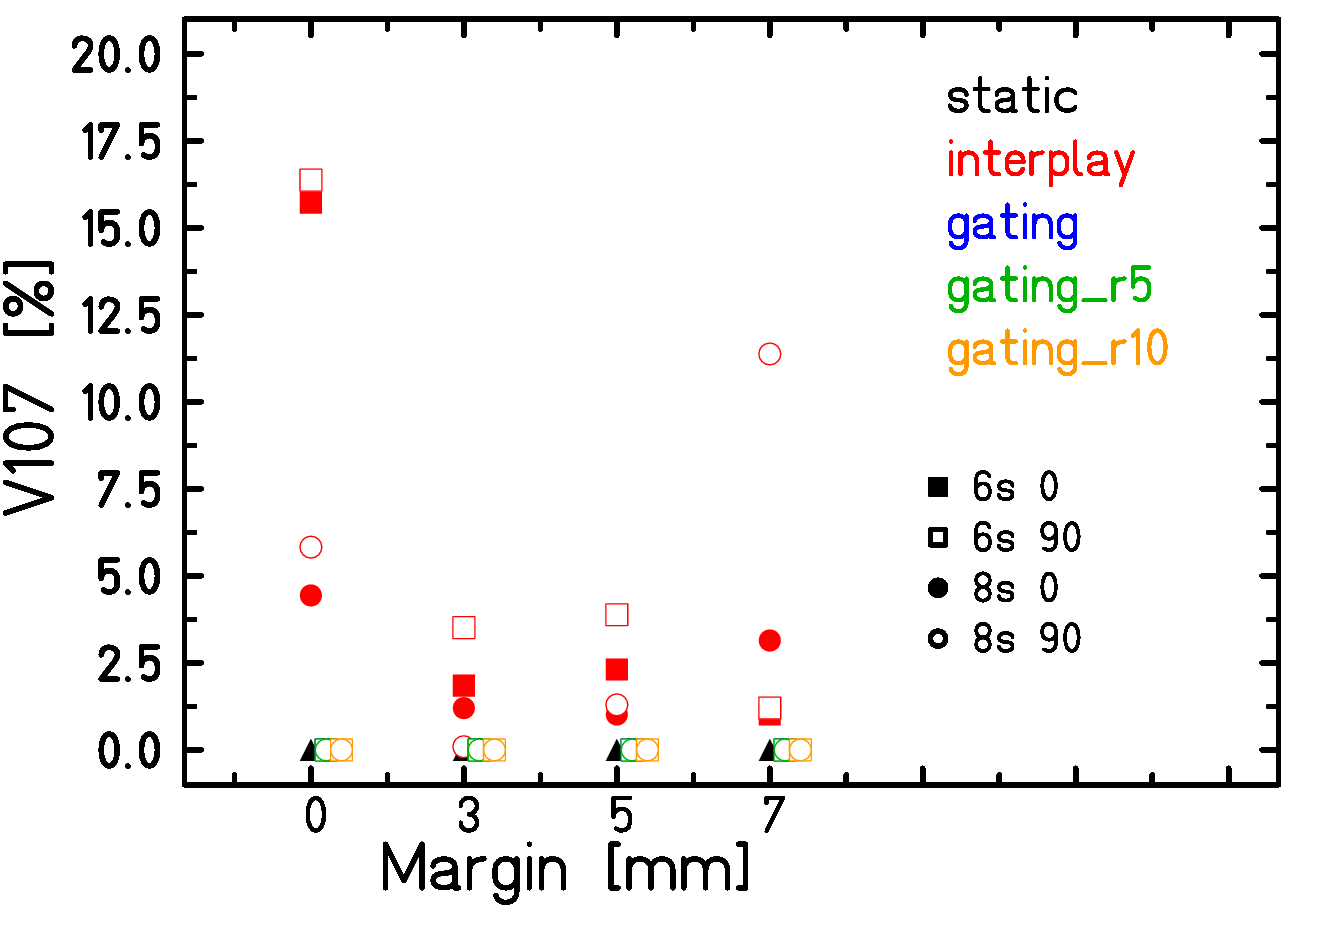
\includegraphics[scale=0.18]{./teile/results_mdacc/MDACC_Pat122_CTV_RPV_V107_withRescan.png}
 }
\caption{Patient 9: Dose analysis parameters for LPV (left column) and RPV (right column). Besides static (black), interplay (red) and gating 
(blue) also different rescan numbers on the gated irradiation were applied (five (green) and ten rescans (orange)). The results are compared for four different 
motions and different safety margins. For a better visualization the rescanning data points for each motion pattern are shifted and the result 
for fifteen and twenty rescans are not displayed.}
\label{static_interplay_gating_rescan_Pat09}
\end{figure}

\newpage

 \begin{figure}[H]
 \begin{center}
\subfigure[LPV]{
 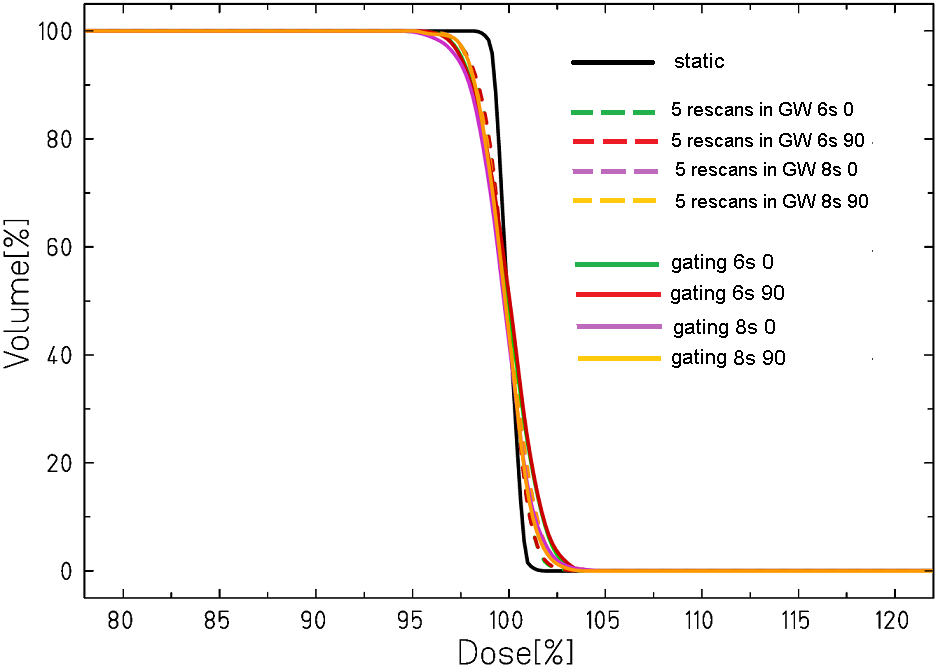
\includegraphics[scale=0.48]{./teile/results_mdacc/Pat09_allDVHs_LPV_rescan_withLegend.png}
 }
\subfigure[RPV]{
 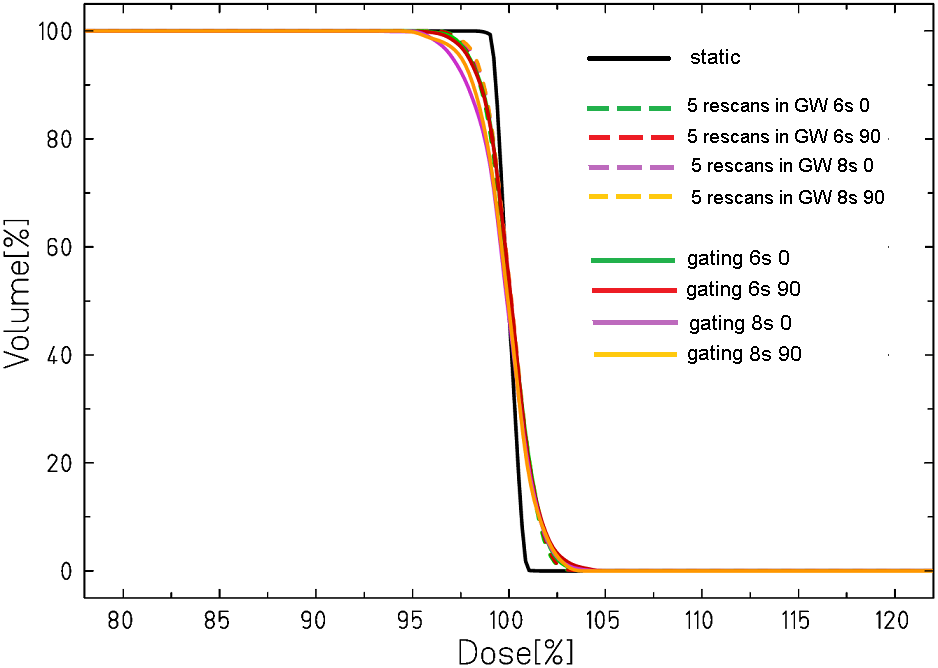
\includegraphics[scale=0.48]{./teile/results_mdacc/Pat09_allDVHs_RPV_rescan_withLegend.png}
 }
\caption{Dose volume histograms for CTV of patient 9 for 3mm safety margin irradiation (LPV (a) as well as RPV (b)) in case of static 
irradiation (black), gating (solid) and five rescans inside the gating window (dashed). The motion patterns are shown in colors (6s 0: lujan motion with period of 6s 
and starting phase 0$^{\circ}$, 6s 90: lujan motion period of 6s and starting phase 90$^{\circ}$, 8s 0: lujan motion period of 8s 
and starting phase 0$^{\circ}$, 8s 90: lujan motion period of 8s and starting phase 90$^{\circ}$.}
\label{dvhs_pat09_mdacc_rescan}
 \end{center}
\end{figure}

\newpage

\begin{figure}[H]
\subfigure[D5-D95: LPV]{
 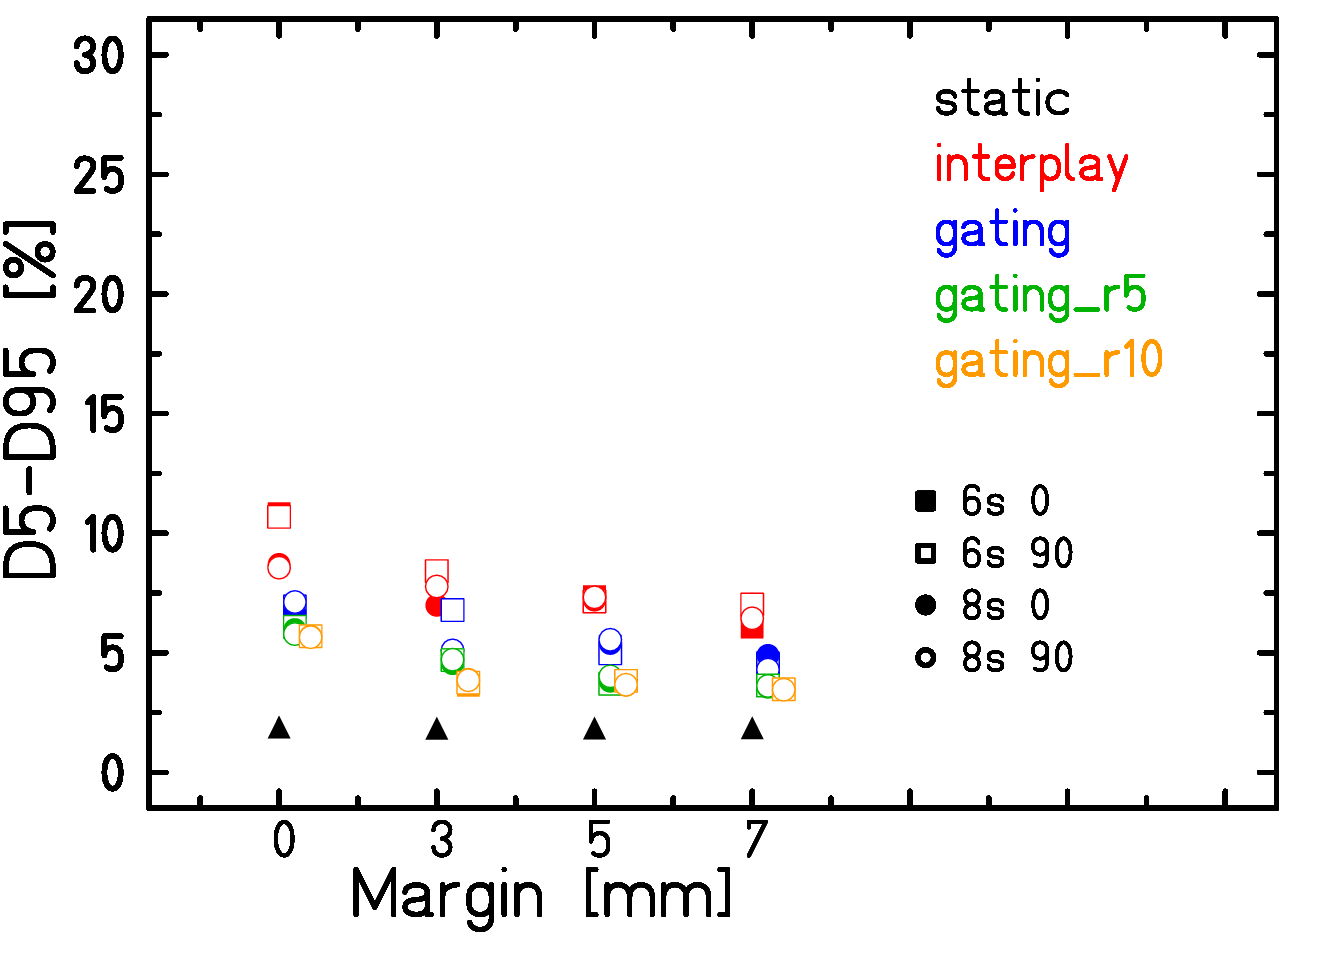
\includegraphics[scale=0.18]{./teile/results_mdacc/MDACC_Pat024_CTV_LPV_D5D95_withRescan.png}
 }
 \subfigure[D5-D95: RPV]{
 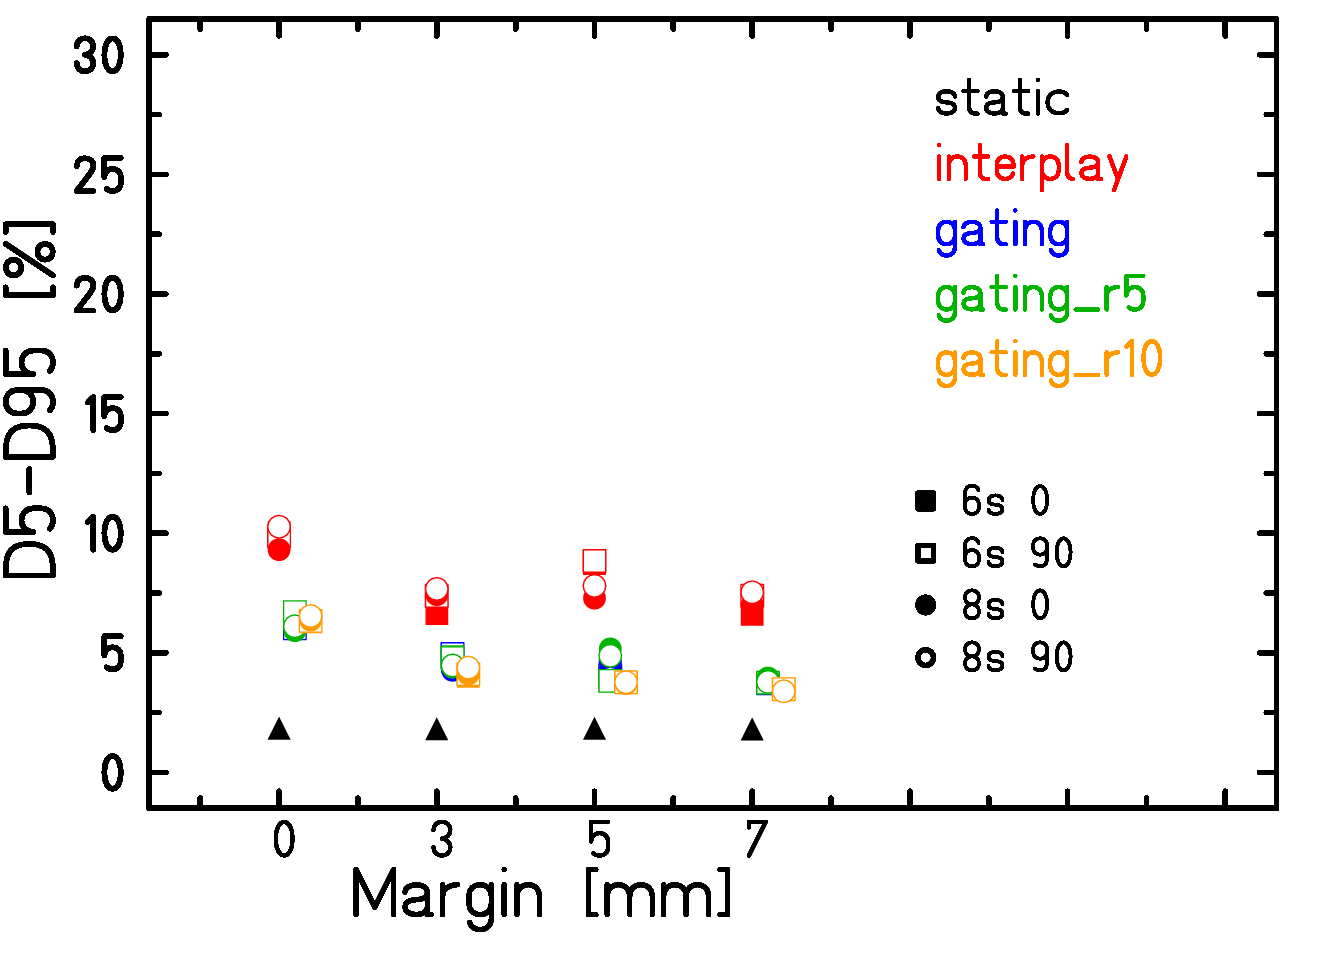
\includegraphics[scale=0.18]{./teile/results_mdacc/MDACC_Pat024_CTV_RPV_D5D95_withRescan.png}
 }
 \subfigure[V95: LPV]{
 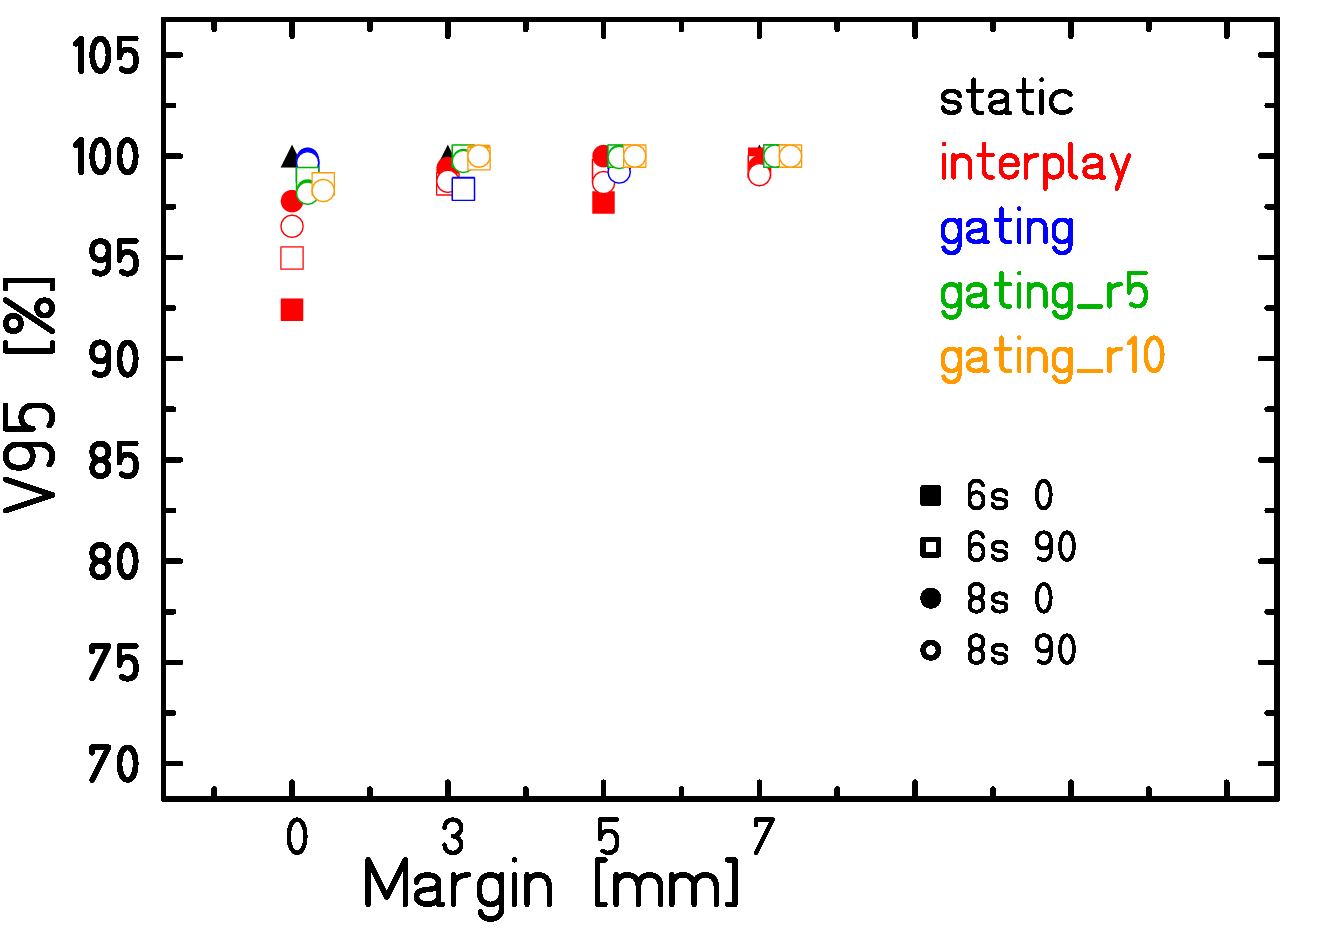
\includegraphics[scale=0.18]{./teile/results_mdacc/MDACC_Pat024_CTV_LPV_V95_withRescan.png}
 }
\subfigure[V95: RPV]{
 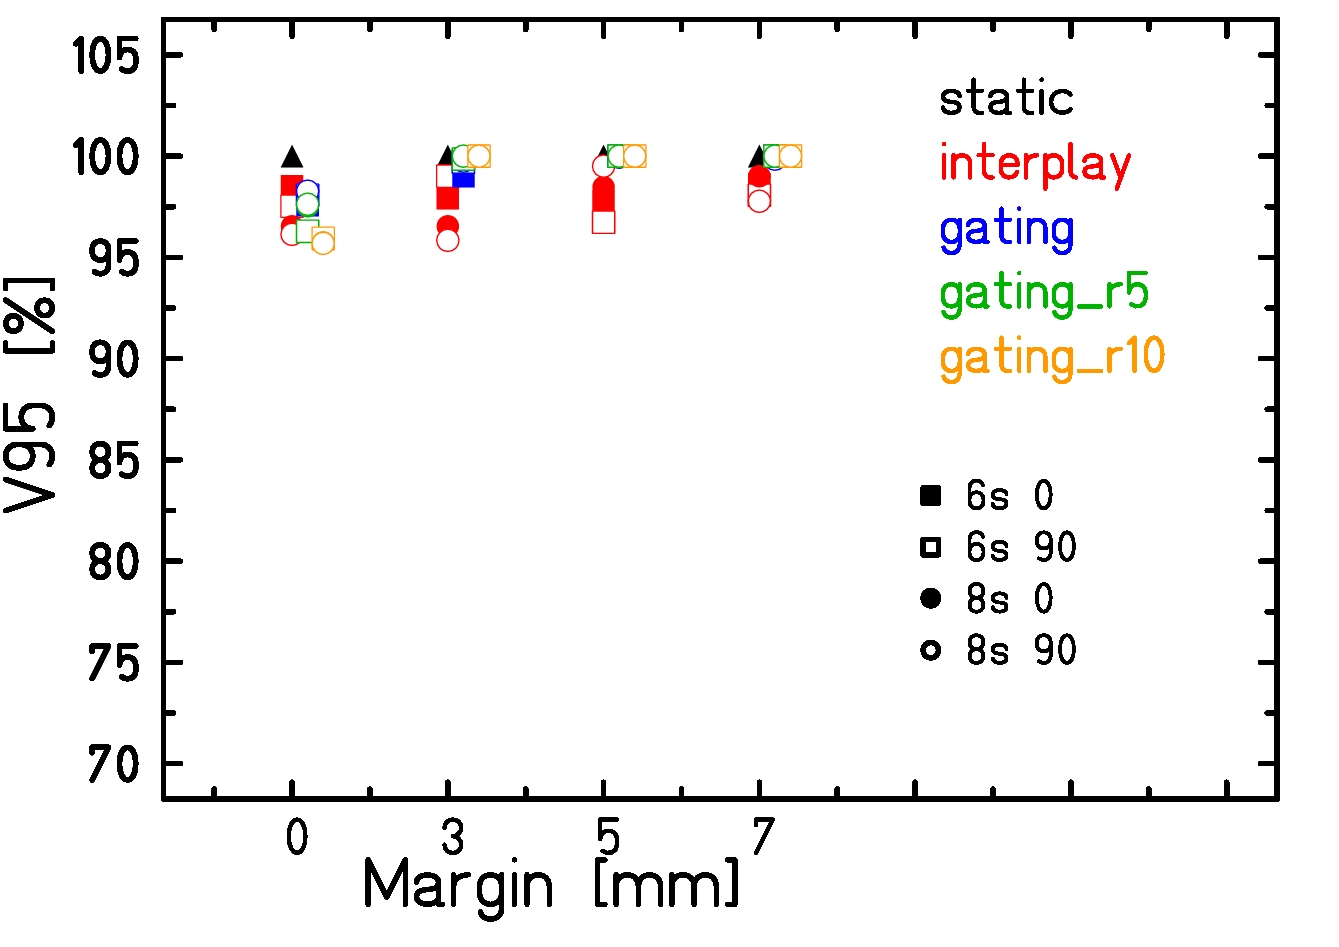
\includegraphics[scale=0.18]{./teile/results_mdacc/MDACC_Pat024_CTV_RPV_V95_withRescan.png}
 }
  \subfigure[V107: LPV]{
 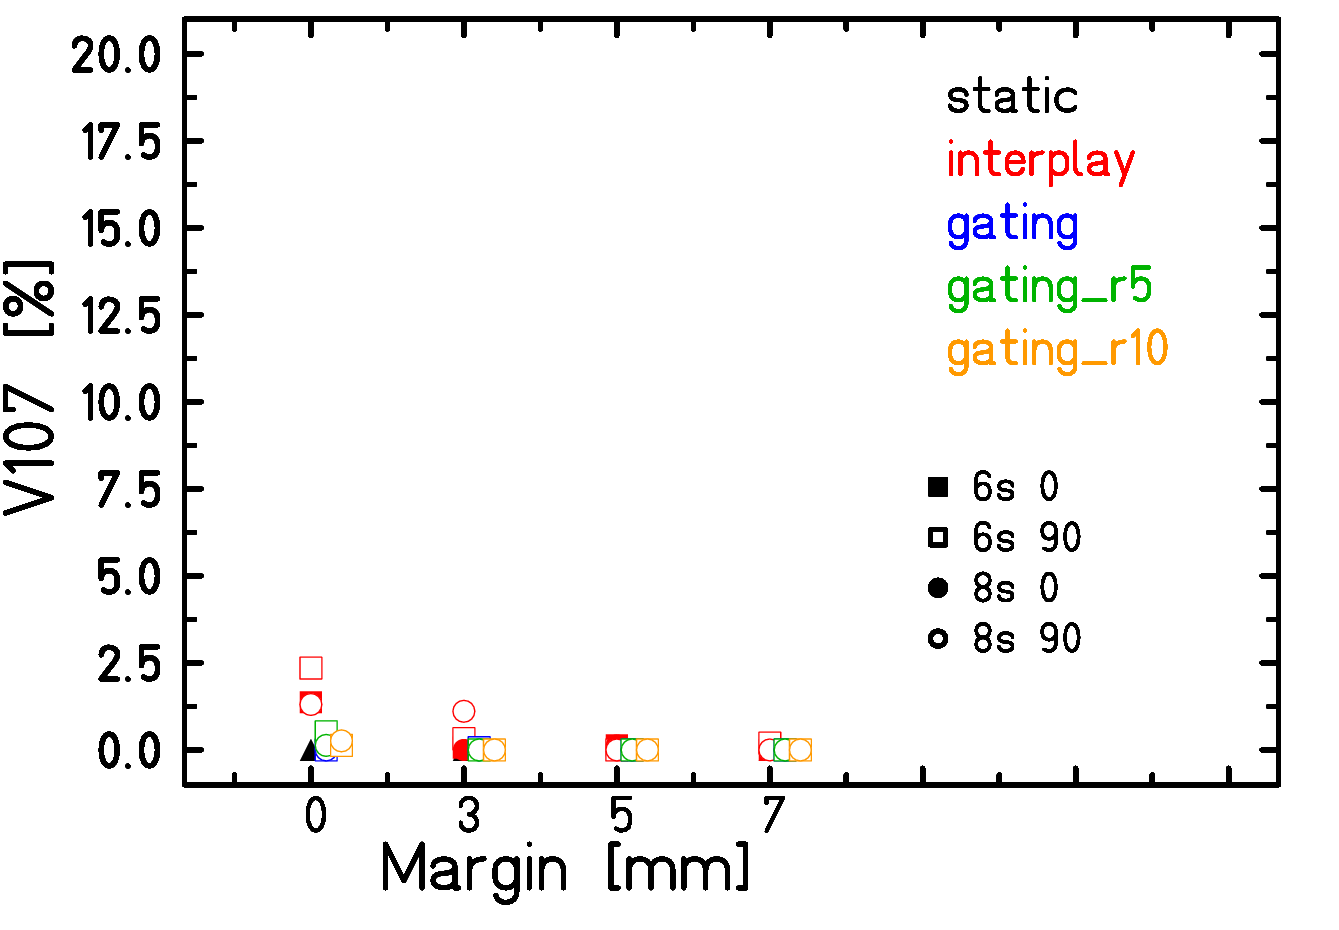
\includegraphics[scale=0.18]{./teile/results_mdacc/MDACC_Pat024_CTV_LPV_V107_withRescan.png}
 }
\subfigure[V107: RPV]{
 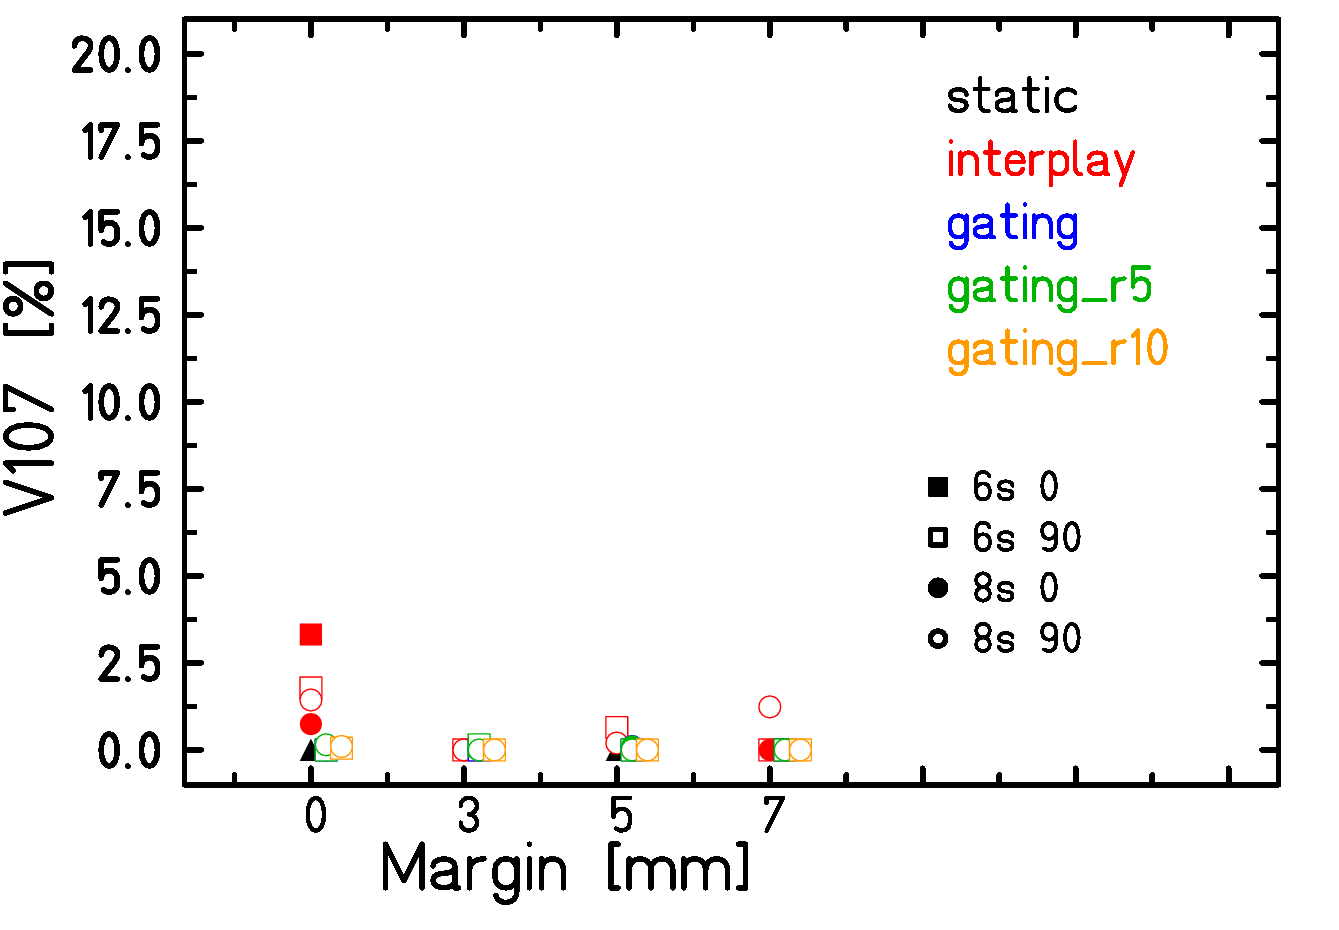
\includegraphics[scale=0.18]{./teile/results_mdacc/MDACC_Pat024_CTV_RPV_V107_withRescan.png}
 }
\caption{Patient 2: Dose analysis parameters for LPV (left column) and RPV (right column). Besides static (black), interplay (red) and gating 
(blue) also different rescan numbers on the gated irradiation were applied (five (green) and ten rescans (orange)). The results are compared 
for four different motions and different safety margins. For a better visualization the rescanning data points for each motion pattern are 
shifted and the result for fifteen and twenty rescans are not displayed.}
\label{static_interplay_gating_rescan_Pat02}
\end{figure}

\newpage


\subsubsection{Irradiation time}

One of the disadvantages of gating as motion mitigation technique is that the irradiation time is increased depending on the used gating window 
size. When a gating window of roughly 30\% is used, like in this study, the irradiation is prolonged by a factor of three compared to the static 
irradiation. In figure \ref{irrTime_gating_Pat024} the needed irradiation time for the gated irradiation of LPV and RPV in patient 2 is shown for 
different safety margins and motion patterns. The duration for each beam entry channel (gantry angle of -45$^{\circ}$, 135$^{\circ}$ and 0$^{\circ}$) 
is plotted individually. On the left side the duration of an irradiation with a small minimal particle number (11,000 particles per beam spot) 
is shown, while on the right side an irradiation with a higher minimal particle number (55,000 particles per beam spot) is displayed. 
Even though a higher intensity is expected to result in a shorter treatment time and would hence be favorable for the efficiency of the 
treatment, it was shown that very high intensities endanger a homogenous dose coverage \cite{Mue14}. The usage of lower intensities is 
hence motivated and needs to be studied in the individual cases.\newline
\newline
As expected, the needed irradiation time increases with the used safety margin as the irradiated volume increases. Furthermore 
the irradiation time is independent of the motion pattern but varies depending on the used beam entry channel. While the low intensity 
irradiation can take up to 120 minutes (for a safety margin of 3mm), the overall duration can be reduced to only 30 minutes (for a safety 
margin of 3mm) for the irradiation with a higher intensity. It should be noted that this is the gating time for the respiratory motion alone 
and the overall treatment time will thus be prolonged, as cardiac motion is not yet compensated for. 

\vspace*{0.6cm}

 \begin{figure}[H]
\subfigure[Patient 2: $N_{\mathrm{min}}$ = 11,000]{
 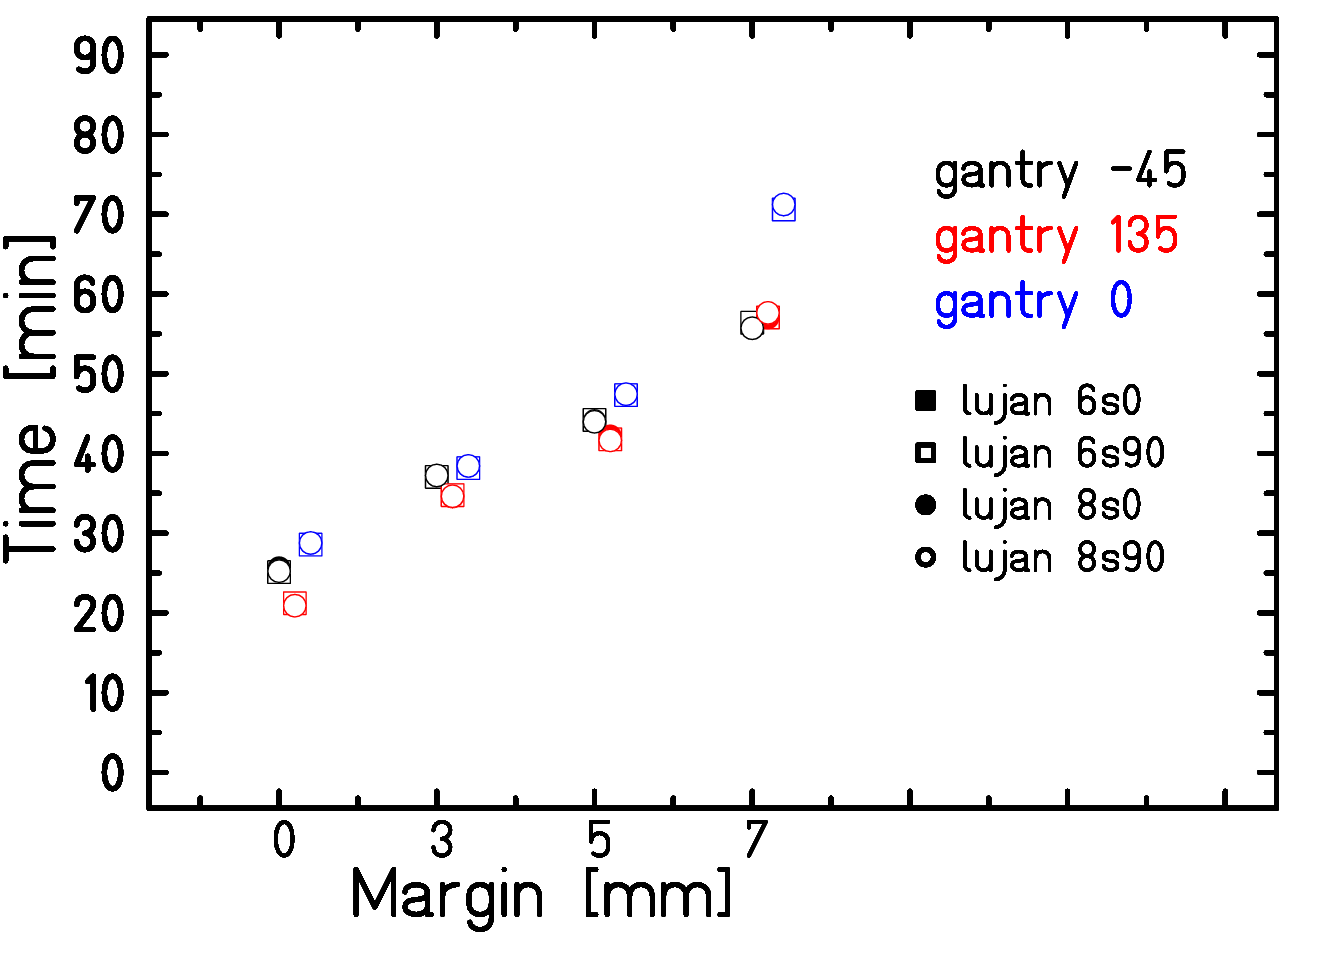
\includegraphics[scale=0.18]{./teile/results_mdacc/Pat024_all_irrTime.png}
 }
\subfigure[Patient 2: $N_{\mathrm{min}}$ = 55,000]{
 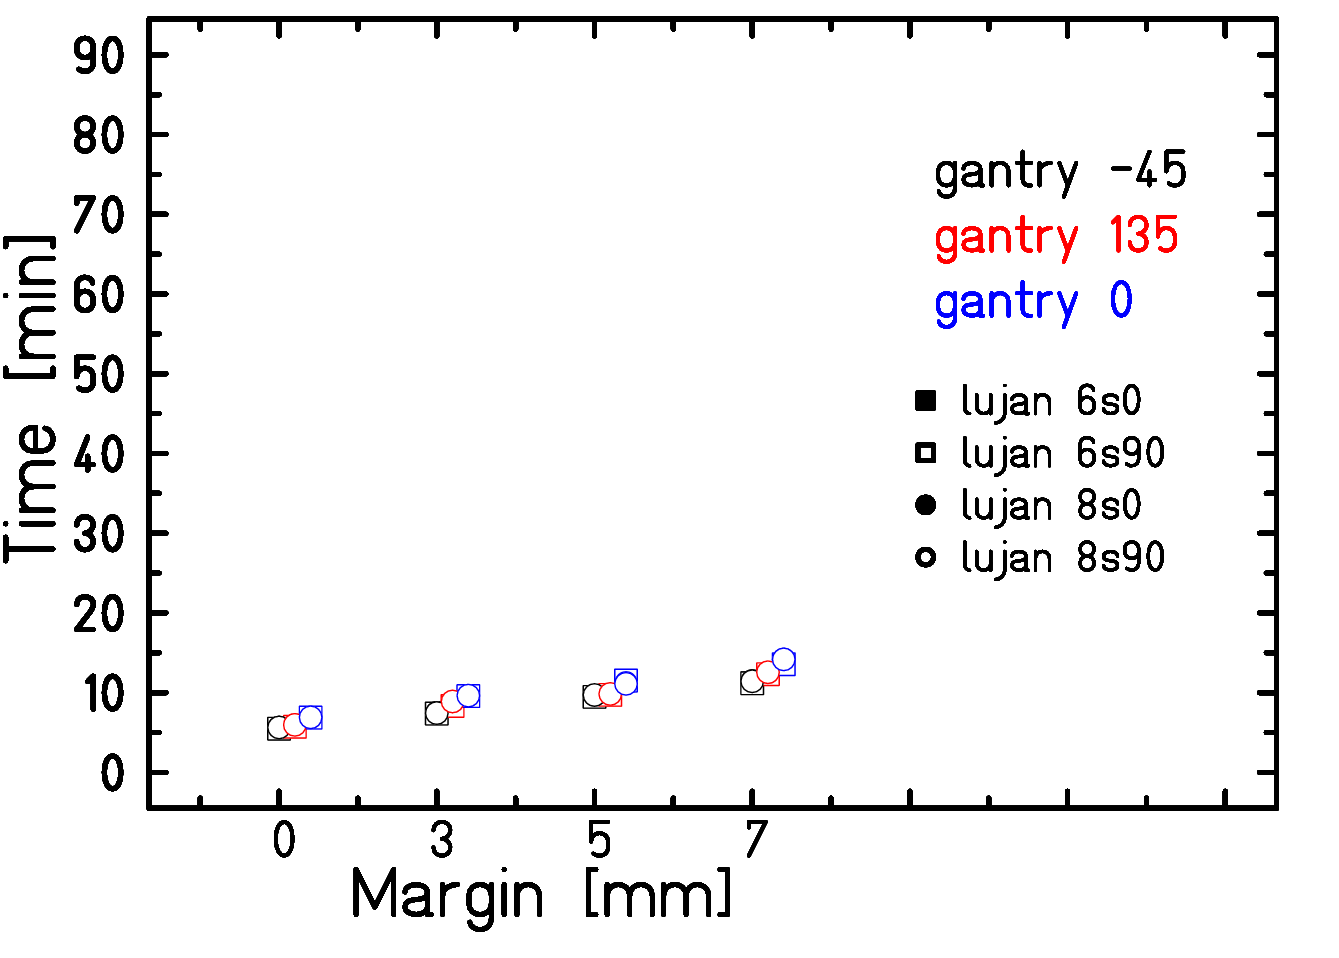
\includegraphics[scale=0.18]{./teile/results_mdacc/Pat024_all_irrTime_hoheNmin.png}
 }
\caption{Irradiation time for gating for patient 2 for different intensities, different 
safety margins, underlying motion patterns and beam entry channels.}
\label{irrTime_gating_Pat024}
\end{figure}



\newpage

\section{Discussion}
In this chapter the influence of respiratory motion on the PVs was studied and treatment planning studies with gating as motion 
mitigation technique were carried out. Respiration was found to be an important motion component for the treatment of cardiac volumes. 
Recent studies in the cardiology community also indicate that real time compensation of breathing displacement 
would even be beneficial for catheter ablation \cite{Kum12, Frie12}.\newline
\newline
Different studies on the influence of respiration on the PV motion exist as they are of interest for image guided ablation procedures. 
Thereby relative displacements (like deformation or splaying of the PVs) and absolute motion (translational and rotation) are distinguished. 
Noseworthy et al. \cite{Nos05} studied the relative changes in the PV anatomy during the breathing cycle. They thereby investigated the changing 
branching angle between the inferior and superior LPV (LIPV, LSPV) and RPV (RIPV, RSPV), respectively. They stated that the PV splay increased 
during inspiration (branching angle of RPVs increased from (40 $\pm$ 10)$^\circ$ to (60 $\pm$ 15)$^\circ$ and for LPVs 
from (50 $\pm$ 11)$^\circ$ to (62 $\pm$ 13)$^\circ$). Furthermore they found a significant reduction in 
the diameter of the RIPV and RSPV during inspiration. Ector et al. \cite{Ect08} on the other hand stated that they only found a slight, 
but significant diameter reduction in the RIPV. In their paper they furthermore studied the absolute translational motion. 
Their patient cohort had a mean diaphragmatic movement of (35 $\pm$ 16)mm for the right diaphragm, resulting in an absolute mean displacement 
for both LPV and RPV of (19.1 $\pm$ 8.6)mm. The mean inferior motion was stated 
to (14.6 $\pm$ 7.7)mm, in anterior direction to (9.7 $\pm$ 7.6)mm and the smallest motion direction was the leftward direction with 
(0.4 $\pm$ 3.8)mm. Comparing motion patterns between veins the LPVs were found to move less in anterior direction then the RPVs, but did 
not differ significantly in other directions. They found a strong association between diaphragmatic motion and inferior PV motion.\newline
\newline
In the here studied patient cohort of lung cancer patients a much smaller mean absolute displacement of the pulmonary veins was found over all 
patients with (6.8 $\pm$ 3.6)mm for LPV and (6.8 $\pm$ 2.5) for RPV. The SI motion had a mean value of (-6.4 $\pm$ 3.8)mm and 
(-6.6 $\pm$ 2.4)mm for RPV, respectively. In AP direction the mean amplitude for all patients was (-0.8 $\pm$ 0.5)mm for LPV and 
(-0.9 $\pm$ 0.8) for RPV, which corresponds to the finding by Ector et al. that the LPV move less in anterior direction than the RPV. For LR 
direction a mean displacement of (-0.9 $\pm$ 0.9) of LPV and (0.5 $\pm$ 1.0)mm of RPV was found over all patients. 
Contrary to Ector et al. a significant difference in the motion of the LPV compared to RPV was hence found in LR. 
A correlation between diaphragm motion and PV displacement was only found in the RPV (r=0.79, p<0.05). Even though a similar result was 
expected for the LPV, no correlation was observed here. It is unclear if this is due to location of the ablation site or due to the 
underlying lung cancer patient data in comparison to AF patient data sets.\newline
\newline
Recent studies in the cardiology community \cite{Kum12} concluded that also for catheter ablation respiration plays an important role as it may 
reduce the catheter tip contact force. Consideration of respiratory motion is thus recommended. Besides ventilation and apnea, Friedmann 
\cite{Frie12} also states that jet ventilation or breath-hold might be adequate strategies for catheter ablation. Even though these techniques 
may also be options for a non-invasive treatment of atrial fibrillation with a scanned carbon ion beam, gating was 
studied as a motion mitigation technique in the present work. In irradiation of cardiac volumes in the animal studies carried out 
at CyberHeart and at the Universit\"atsklinikum Schleswig-Holstein in L\"ubeck different approaches were used. While Blanck et al. 
\cite{Bla13} used an ITV approach for the respiratory motion, Sharma et al. \cite{Sha10} tracked the respiration with the underlying 
CyberKnife Synchrony software (see chapter \ref{chapter:intro}, section \ref{Motionacq}). For particle therapy tracking is not feasible yet as 
no fast and precise real-time internal motion monitoring including particle range information exists. A simple enlargement of internal margins 
to produce an ITV for respiration was withdrawn due to expected high dose deposition in critical OAR close to the target sites 
(see chapter \ref{chapter:human}). Gating offers the advantage of a currently technical feasibility while keeping the dose to the normal 
tissue relatively small. Nevertheless it leads to a prolongation of the treatment time. However, with a high intensity of 55,000 minimum 
particles per spill a duration of only 30 minutes could be achieved (patient 2, safety margin of 3mm). This already offers a reduced 
treatment time compared to the results by Sharma et al. where a treatment time of one to two hours was estimated. 
While lower intensities lead to a longer treatment time, it is nevertheless known from previous studies \cite{Mue14} that high intensities 
can result in inhomogeneous dose depositions. Other methods to reduce the treatment time might hence be needed in order to still guarantee a time 
efficient delivery. Tsunashima et al. \cite{Tsu08} studied cyclotron settings that could lead to a reduced treatment time in particle gating. 
They thereby found that variable excitation cycles, in synchrony with the respiratory pattern of the patient, could reduce the treatment time 
prolongation to a factor two, instead of the usual factor three, for a 30\% gating window. 
Iwata et al. \cite{Iwa10b} furthermore proposed a method to reduce the needed time for energy changes inbetween IESs in synchrotrons. 
By using radiofrequency knockout exciters and multiple energy operation patterns, the beam would be accelerated to the maximum energy and than 
stepwise decelerated to lower energies, using an extension of the respective flattops to extract the particles with varying energies during a 
single operation cycle of the synchrotron.\newline
\newline
Concerning the dose deposition with gating compared to interplay it can be concluded that gating yields good dose coverage. The V95 values 
were higher than 99\% for all target sites with safety margin of 3mm or more and higher than 95\% in all cases without safety margin (minimum of 
95.21\% in patient 9 for LPV, no safety margin and motion period of 8s, starting phase of 0$^{\circ}$).The V107 values were all smaller 
than 0.1\% (maximum of 0.1\% for patient 2, RPV, in case of 5mm margin and motion with period of 8s and starting phase of 90$^{\circ}$). 
Hence an acceptable dose coverage could be achieved. The dose homogeneity did not exceed 9.18\% without safety margin (patient 5, LPV, no 
safety margin and motion period of 8s, starting phase of 90$^{\circ}$). With safety margin, the D5-D95 value did not exceed 8\%. An additional 
safety margin is thus beneficial to guarantee a robust and successful treatment delivery. However, an extension of the target volume due to 
safety margins always results in more dose to the normal tissue and to potential critical OARs. A limited safety margin of 3mm or 5mm would 
offer the benefit of improved treatment outcome while keeping the irradiated volume low (see also chapter \ref{chapter:human}).\newline
\newline
Rescanning within the gating window could slightly improve the results for dose homogeneity as it reduces the influence of residual motion 
inside the gating window. The dose homogeneity in the LPV of patient 9 for example (large motion amplitude) could be reduced from 5.01\%  
(safety margin of 3mm, motion period 6s and 90$^{\circ}$ starting phase) to 3.83\% with five rescans. 


\section{Conclusion}

The PVs were found to move due to respiration with an amplitude of up to 2cm. 
This displacement creates interplay effects when irradiated with scanned carbon ions. Gating as motion mitigation technique was studied. 
It can be concluded that this method yields improved dose coverage (under and over dosage) and better dose homogeneity compared to interplay 
in all studied patient cases, for all motion patterns and safety margins and achieves results comparable to the static irradiations. 
It can thus be an adequate motion mitigation technique for the irradiation of PVs under influence of respiratory motion. 
As rescanning is a potential technique when compensating for displacements due to 
heartbeat (see chapter \ref{chapter:human}), the combination of these two motion mitigation technique could be feasible in a potential 
application. Hence rescanning inside the gating window was studied and it was shown that a  small number of rescans (e.g. five or ten) are 
sufficient to improve the results of dose homogeneity. 



%%%%%%%%%%%%%%%%%%%%%%%%%%%%%%%%%%%%%%%%%%%
%%%%%%%%%%%%%% APPENDIX %%%%%%%%%%%%%%%%%%%
%%%%%%%%%%%%%%%%%%%%%%%%%%%%%%%%%%%%%%%%%%%


